\documentclass[aspectratio=169, 12pt]{beamer}

% Theme
\usetheme{default}
\usecolortheme{whale}
\setbeamertemplate{navigation symbols}{}
\setbeamertemplate{footline}[frame number]

% Packages
\usepackage{graphicx}
\usepackage{booktabs}
\usepackage{amsmath}
\usepackage{xcolor}
\usepackage{tikz}
\usetikzlibrary{positioning, shapes.geometric}

% Colors
\definecolor{mainblue}{HTML}{2D5F91}
\definecolor{accentred}{HTML}{D65F5F}
\definecolor{accentgreen}{HTML}{4CAF50}
\definecolor{lightgray}{HTML}{F5F5F5}
\setbeamercolor{frametitle}{fg=mainblue}
\setbeamercolor{title}{fg=mainblue}
\setbeamercolor{alerted text}{fg=accentred}

% Figure path
\graphicspath{{figures/}}

% Metadata
\title{Imputing Cell Expression from Single-Nucleus RNA-seq\\with a Modality-Conditioned VAE}
\author{Shaoqian Zhang}
\institute{Gerstein Lab, Yale University}
\date{Lab Meeting --- April 3, 2026}

\begin{document}

% ============================================================
% SLIDE 1: Title
% ============================================================
\begin{frame}[plain]
\maketitle
\end{frame}

% ============================================================
% SECTION 1: THE PROBLEM
% ============================================================
\section{The Problem}

% ============================================================
% SLIDE 2: snRNA-seq is incomplete
% ============================================================
\begin{frame}{Single-Nucleus Sequencing Misses Cytoplasmic RNA}
\begin{columns}[T]
\begin{column}{0.55\textwidth}
\begin{itemize}
    \item PsychENCODE: \textbf{2.8M nuclei}, 388 brains {\small (Gerstein, \textit{Science} '24)}
    \item Nuclei lack cytoplasmic mRNA: activity genes (\textit{Fos}, \textit{Arc}), secreted factors
    \item Population-level cell--nucleus correlation $r \approx 0.82$
\end{itemize}
\end{column}
\begin{column}{0.42\textwidth}
\centering
% Placeholder for cell schematic
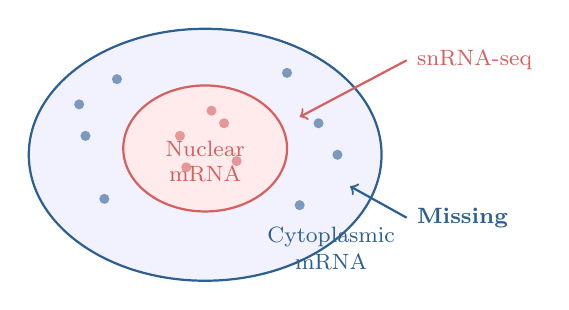
\begin{tikzpicture}[scale=0.8]
    % Cell
    \draw[thick, mainblue, fill=blue!5] (0,0) ellipse (2.8 and 2);
    % Nucleus
    \draw[thick, accentred, fill=red!8] (0,0.1) ellipse (1.3 and 1);
    % Labels
    \node[mainblue, font=\footnotesize] at (2.0, -1.3) {Cytoplasmic};
    \node[mainblue, font=\footnotesize] at (2.0, -1.7) {mRNA};
    \node[accentred, font=\footnotesize] at (0, 0.1) {Nuclear};
    \node[accentred, font=\footnotesize] at (0, -0.3) {mRNA};
    % RNA dots - cytoplasmic
    \foreach \x/\y in {1.8/0.5, -1.9/0.3, 1.5/-0.8, -1.6/-0.7, 2.1/0, -2.0/0.8, 1.3/1.3, -1.4/1.2}{
        \fill[mainblue, opacity=0.6] (\x,\y) circle (0.08);
    }
    % RNA dots - nuclear
    \foreach \x/\y in {0.3/0.5, -0.4/0.3, 0.5/-0.1, -0.3/-0.2, 0.1/0.7}{
        \fill[accentred, opacity=0.6] (\x,\y) circle (0.08);
    }
    % snRNA-seq bracket
    \draw[<-, thick, accentred] (1.5, 0.6) -- (3.2, 1.5) node[right, font=\footnotesize] {snRNA-seq};
    \draw[<-, thick, mainblue] (2.3, -0.5) -- (3.2, -1.0) node[right, font=\footnotesize] {\textbf{Missing}};
\end{tikzpicture}
\end{column}
\end{columns}
\end{frame}

% ============================================================
% SLIDE 3: Can we recover cell expression?
% ============================================================
\begin{frame}{Predicting Whole-Cell Profiles from Nuclei Alone}
\begin{itemize}
    \item Allen Brain Atlas: \textbf{17 cell types}, $\sim$71K cells + $\sim$40K nuclei (v3, unpaired)
    \item No matched cell--nucleus pairs --- learn from population correspondence
    \item Goal: nucleus profile $\xrightarrow{\text{VAE}}$ cell-like profile
\end{itemize}

\vspace{0.5em}
\centering
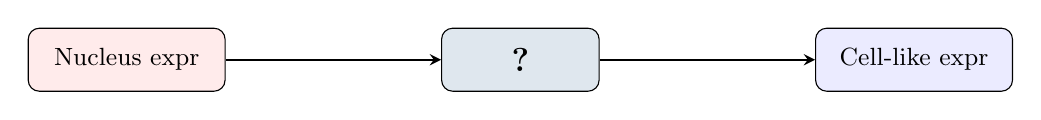
\begin{tikzpicture}[>=stealth, font=\small]
    \node[draw, rounded corners, fill=red!8, minimum width=2.5cm, minimum height=0.8cm] (nuc) at (0,0) {Nucleus expr};
    \node[draw, rounded corners, fill=mainblue!15, minimum width=2cm, minimum height=0.8cm, font=\large\bfseries] (vae) at (5,0) {?};
    \node[draw, rounded corners, fill=blue!8, minimum width=2.5cm, minimum height=0.8cm] (cell) at (10,0) {Cell-like expr};
    \draw[->, thick] (nuc) -- (vae);
    \draw[->, thick] (vae) -- (cell);
\end{tikzpicture}
\end{frame}

% ============================================================
% SECTION 2: APPROACH
% ============================================================
\section{Approach}

% ============================================================
% SLIDE 4: VAE primer
% ============================================================
\begin{frame}{Variational Autoencoder in 60 Seconds}
\begin{itemize}
    \item Encoder: 10K genes $\rightarrow$ 32-dim latent $z$; Decoder: $z \rightarrow$ reconstructed expression
    \item $\mathcal{L} = \mathcal{L}_{\text{recon}}(\text{MSE on log1p}) + \beta \cdot D_{\text{JSD}}(q(z) \,\|\, p(z))$
    \item MSE on log1p outperformed negative binomial (softmax bottleneck)
\end{itemize}

\vspace{0.5em}
\centering
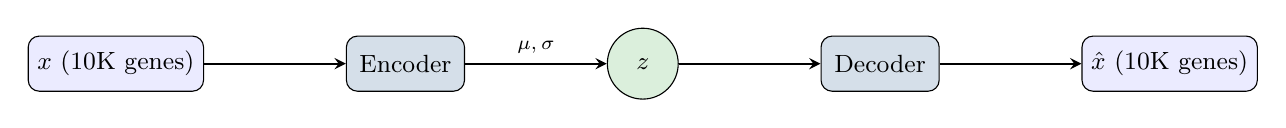
\begin{tikzpicture}[>=stealth, font=\small, node distance=1.8cm]
    \node[draw, rounded corners, fill=blue!8, minimum width=1.8cm, minimum height=0.7cm] (input) {$x$ (10K genes)};
    \node[draw, rounded corners, fill=mainblue!20, minimum width=1.5cm, minimum height=0.7cm, right=of input] (enc) {Encoder};
    \node[draw, circle, fill=accentgreen!20, minimum size=0.9cm, right=of enc] (z) {$z$};
    \node[draw, rounded corners, fill=mainblue!20, minimum width=1.5cm, minimum height=0.7cm, right=of z] (dec) {Decoder};
    \node[draw, rounded corners, fill=blue!8, minimum width=1.8cm, minimum height=0.7cm, right=of dec] (output) {$\hat{x}$ (10K genes)};
    \draw[->, thick] (input) -- (enc);
    \draw[->, thick] (enc) -- (z) node[midway, above, font=\scriptsize] {$\mu, \sigma$};
    \draw[->, thick] (z) -- (dec);
    \draw[->, thick] (dec) -- (output);
\end{tikzpicture}
\end{frame}

% ============================================================
% SLIDE 5: Conditioned decoder
% ============================================================
\begin{frame}{One Decoder, Two Modes --- Learned Modality Embedding}
\begin{itemize}
    \item Shared encoder maps both modalities into aligned latent space
    \item Decoder input: $[\,z \;\|\; e_{\text{mod}}\,]$ with learned 8-dim modality embedding
    \item \textbf{The trick}: encode nucleus $\rightarrow$ decode with \alert{cell embedding} $\rightarrow$ cell-like output
\end{itemize}

\vspace{0.3em}
\centering
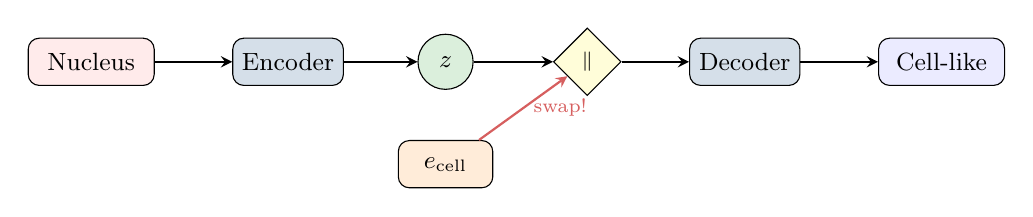
\begin{tikzpicture}[>=stealth, font=\small, node distance=1.2cm]
    % Encoder
    \node[draw, rounded corners, fill=red!8, minimum width=1.6cm, minimum height=0.6cm] (nuc) at (0,0) {Nucleus};
    \node[draw, rounded corners, fill=mainblue!20, minimum width=1.4cm, minimum height=0.6cm] (enc) at (2.5,0) {Encoder};
    \node[draw, circle, fill=accentgreen!20, minimum size=0.7cm] (z) at (4.5,0) {$z$};

    % Concat
    \node[draw, rounded corners, fill=orange!15, minimum width=1.2cm, minimum height=0.6cm] (emb) at (4.5,-1.3) {$e_{\text{cell}}$};
    \node[draw, diamond, fill=yellow!15, minimum size=0.5cm, font=\scriptsize] (cat) at (6.3,0) {$\|$};

    % Decoder
    \node[draw, rounded corners, fill=mainblue!20, minimum width=1.4cm, minimum height=0.6cm] (dec) at (8.3,0) {Decoder};
    \node[draw, rounded corners, fill=blue!8, minimum width=1.6cm, minimum height=0.6cm] (out) at (10.8,0) {Cell-like};

    \draw[->, thick] (nuc) -- (enc);
    \draw[->, thick] (enc) -- (z);
    \draw[->, thick] (z) -- (cat);
    \draw[->, thick, accentred] (emb) -- (cat) node[midway, right, font=\scriptsize, accentred] {swap!};
    \draw[->, thick] (cat) -- (dec);
    \draw[->, thick] (dec) -- (out);
\end{tikzpicture}
\end{frame}

% ============================================================
% SLIDE 6: Cascading losses
% ============================================================
\begin{frame}{Staged Training: Losses Activate Sequentially}
\begin{itemize}
    \item Stage 1: pretrain on cell data only (600 epochs)
    \item Stage 2: cascading annealing prevents decoder degradation
    \item Simultaneous losses degraded decoder in earlier attempts
\end{itemize}

\vspace{0.4em}
\centering
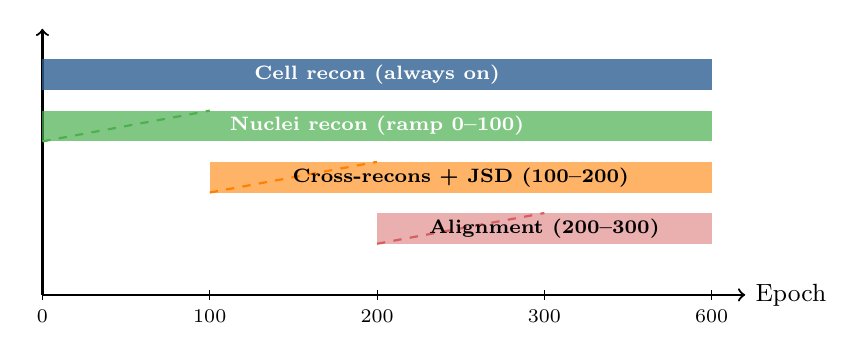
\begin{tikzpicture}[font=\small, yscale=0.65, xscale=0.85]
    % Axis
    \draw[->, thick] (0,0) -- (10.5,0) node[right] {Epoch};
    \draw[->, thick] (0,0) -- (0,5.2);

    % Epoch markers
    \foreach \x/\label in {0/0, 2.5/100, 5/200, 7.5/300, 10/600}{
        \draw (\x, -0.1) -- (\x, 0.1);
        \node[below, font=\scriptsize] at (\x, -0.1) {\label};
    }

    % Bars (Gantt style)
    \fill[mainblue, opacity=0.8] (0, 4) rectangle (10, 4.6);
    \node[white, font=\scriptsize\bfseries] at (5, 4.3) {Cell recon (always on)};

    \fill[accentgreen, opacity=0.7] (0, 3) rectangle (10, 3.6);
    \draw[accentgreen, thick, dashed] (0,3) -- (2.5, 3.6);
    \node[white, font=\scriptsize\bfseries] at (5, 3.3) {Nuclei recon (ramp 0--100)};

    \fill[orange, opacity=0.6] (2.5, 2) rectangle (10, 2.6);
    \draw[orange, thick, dashed] (2.5, 2) -- (5, 2.6);
    \node[font=\scriptsize\bfseries] at (6.25, 2.3) {Cross-recons + JSD (100--200)};

    \fill[accentred, opacity=0.5] (5, 1) rectangle (10, 1.6);
    \draw[accentred, thick, dashed] (5, 1) -- (7.5, 1.6);
    \node[font=\scriptsize\bfseries] at (7.5, 1.3) {Alignment (200--300)};
\end{tikzpicture}
\end{frame}

% ============================================================
% SLIDE 7: Three models
% ============================================================
\begin{frame}{Three Model Variants Compared}

\centering
\begin{tabular}{lccc}
\toprule
 & \textbf{Shared} & \textbf{Cond} & \textbf{Cond+XR} \\
\midrule
Modality embedding & \texttimes & \checkmark & \checkmark \\
Cross-recons loss & \texttimes & \texttimes & \checkmark \\
Cross-decode capable & \texttimes & \checkmark & \checkmark \\
\bottomrule
\end{tabular}

\vspace{1em}
\begin{itemize}
    \item All use MSE loss on log1p data, same architecture (1024$\to$512$\to$32)
    \item Also tested NB loss --- MSE wins (softmax bottleneck distorts proportions)
    \item Shared decoder = baseline; conditioned decoder = key architectural insight
\end{itemize}
\end{frame}

% ============================================================
% SECTION 3: RESULTS
% ============================================================
\section{Results}

% ============================================================
% SLIDE 8: Key unlock
% ============================================================
\begin{frame}{Modality Embedding Enables Cross-Modal Translation}
\begin{columns}[T]
\begin{column}{0.45\textwidth}
\begin{itemize}
    \item Shared: $r = 0.79$, $R^2 = -1.1$\\ {\small (worse than predicting the mean)}
    \item Cond: $r = 0.94$, $R^2 = 0.56$
    \item \textbf{Cond+XR}: $r = 0.98$, $R^2 = 0.95$
\end{itemize}
\end{column}
\begin{column}{0.53\textwidth}
\centering
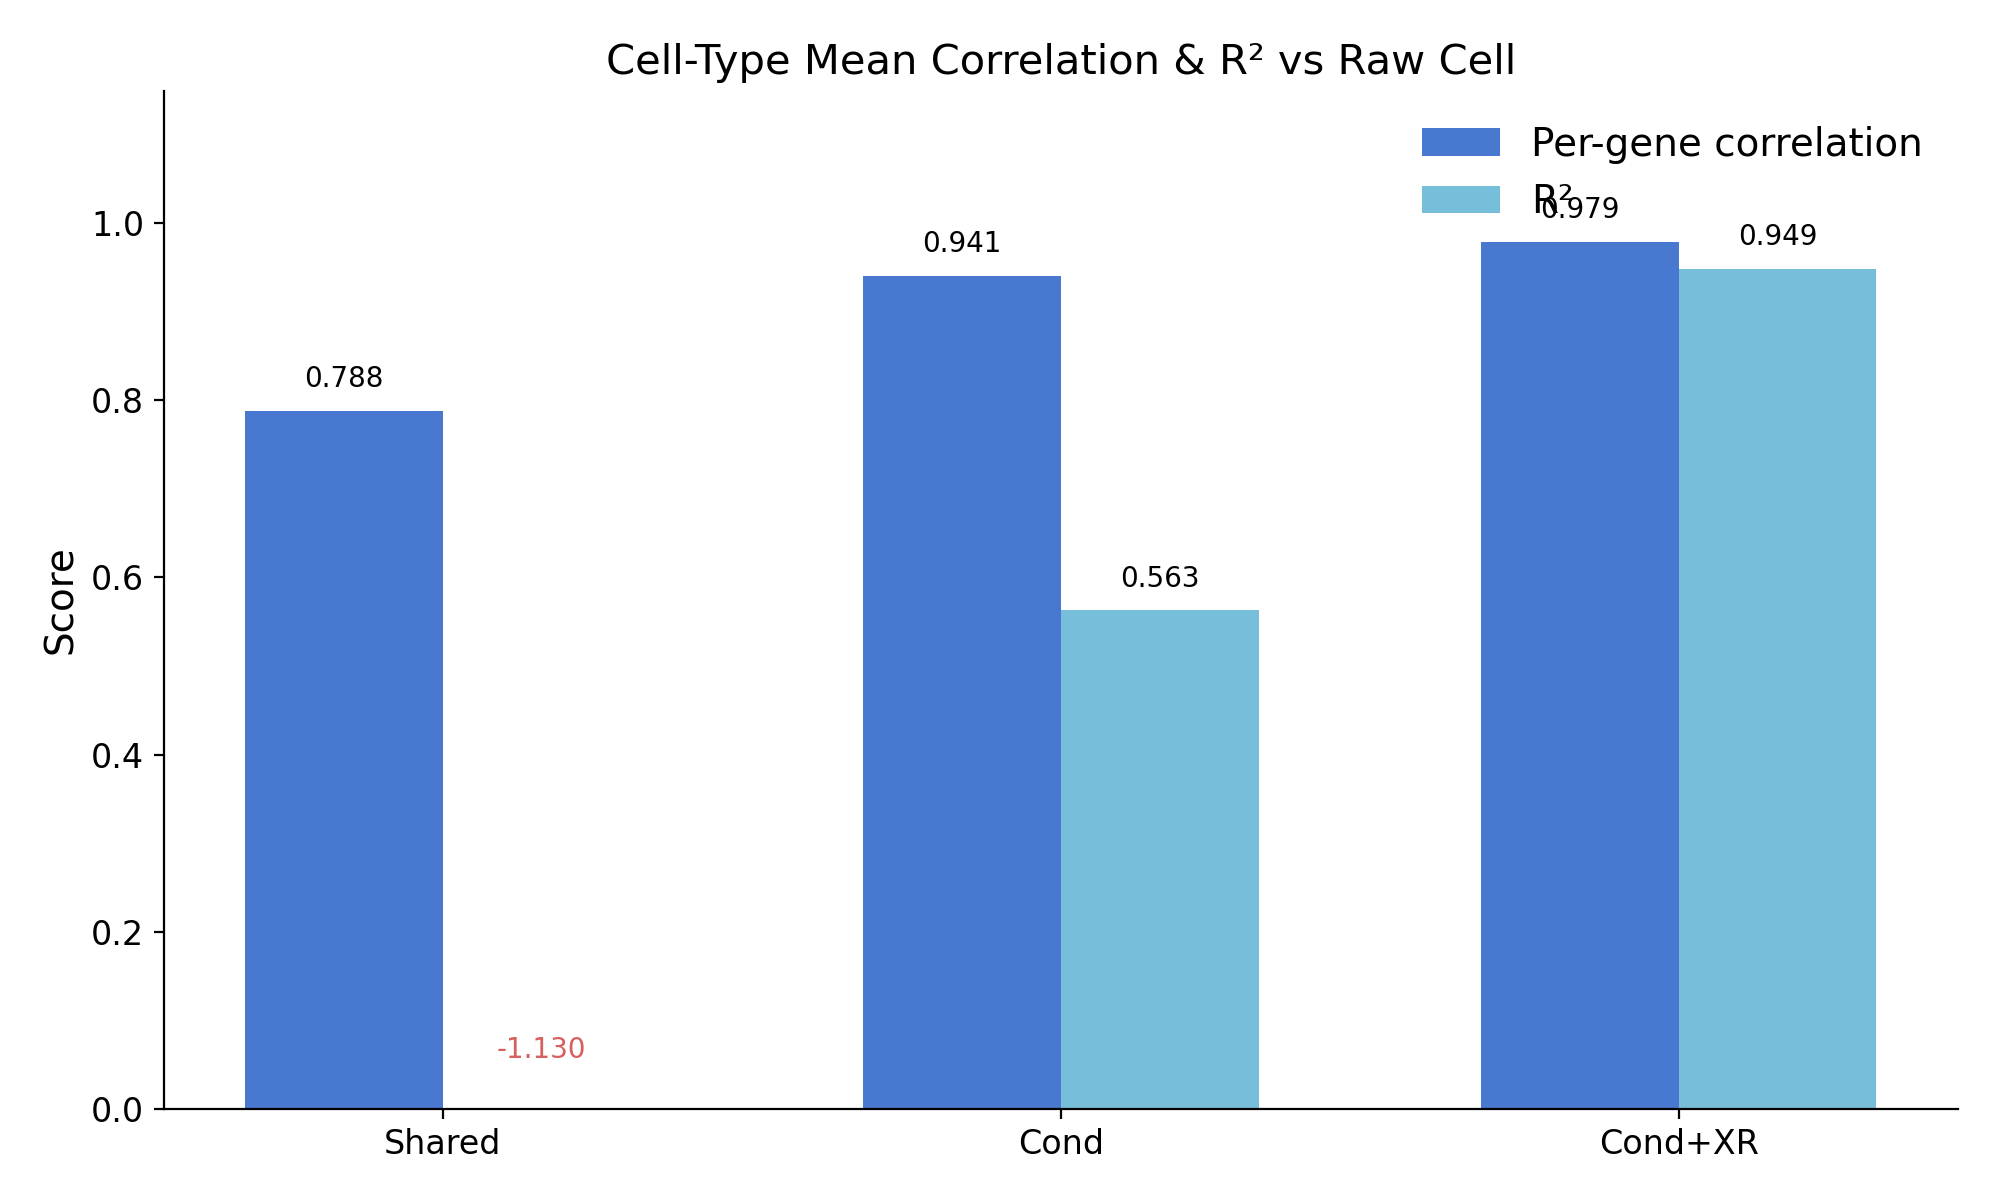
\includegraphics[width=\textwidth]{model_comparison_corr_r2.png}
\end{column}
\end{columns}
\end{frame}

% ============================================================
% SLIDE 9: Classification
% ============================================================
\begin{frame}{Imputed Nuclei Classify Better Than Raw Nuclei}
\begin{columns}[T]
\begin{column}{0.42\textwidth}
\begin{itemize}
    \item Logistic regression trained on real cells
    \item Raw nuclei: 85.1\% accuracy
    \item Imputed (Cond+XR): \textbf{95.8\%} (+10.7\%)
    \item Consistent across neuronal types
\end{itemize}
\end{column}
\begin{column}{0.56\textwidth}
\centering
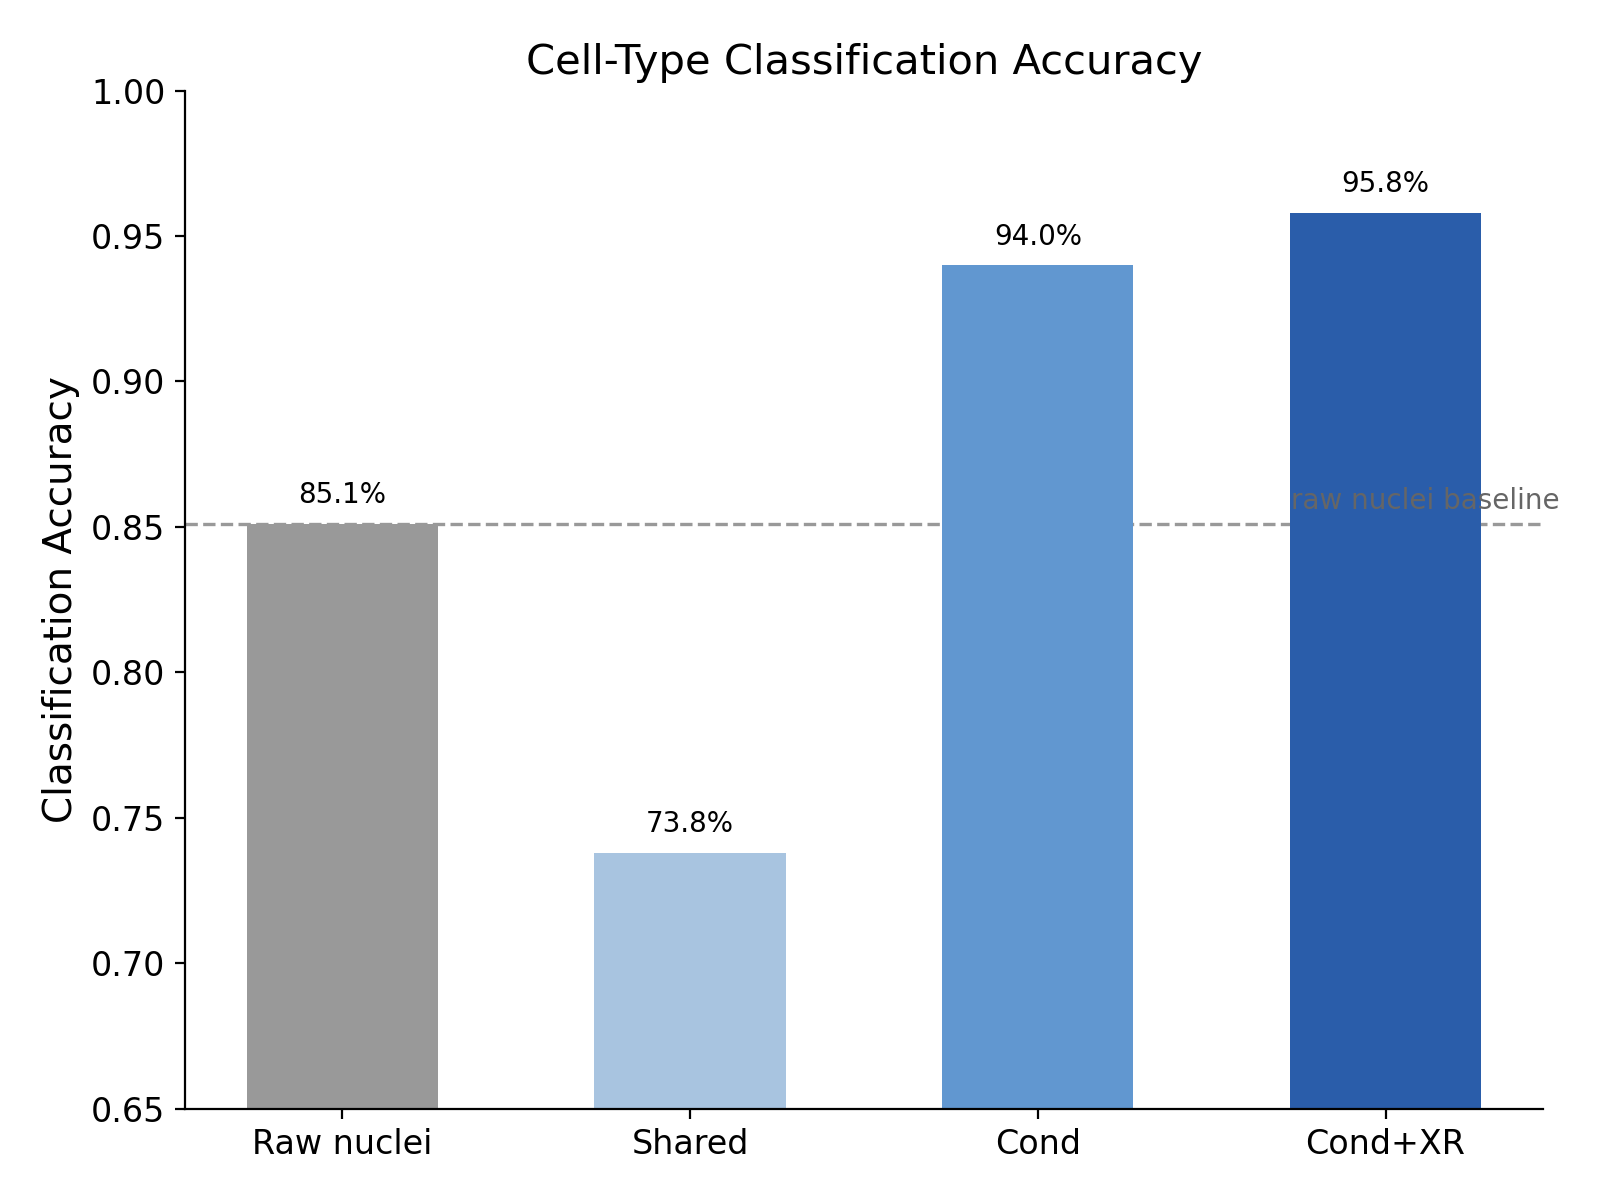
\includegraphics[width=\textwidth]{classification_accuracy.png}
\end{column}
\end{columns}
\end{frame}

% ============================================================
% SLIDE 10: DE recovery
% ============================================================
\begin{frame}{Cross-Decode Recovers More DE Genes Than Raw Nuclei}
\begin{columns}[T]
\begin{column}{0.35\textwidth}
\begin{itemize}
    \item Top-100 Wilcoxon DE: imputed \textbf{52\%} vs raw 47\%
    \item 11/17 types improved
    \item Recon ceiling 55\% --- cross-decode nearly matches
\end{itemize}
\end{column}
\begin{column}{0.63\textwidth}
\centering
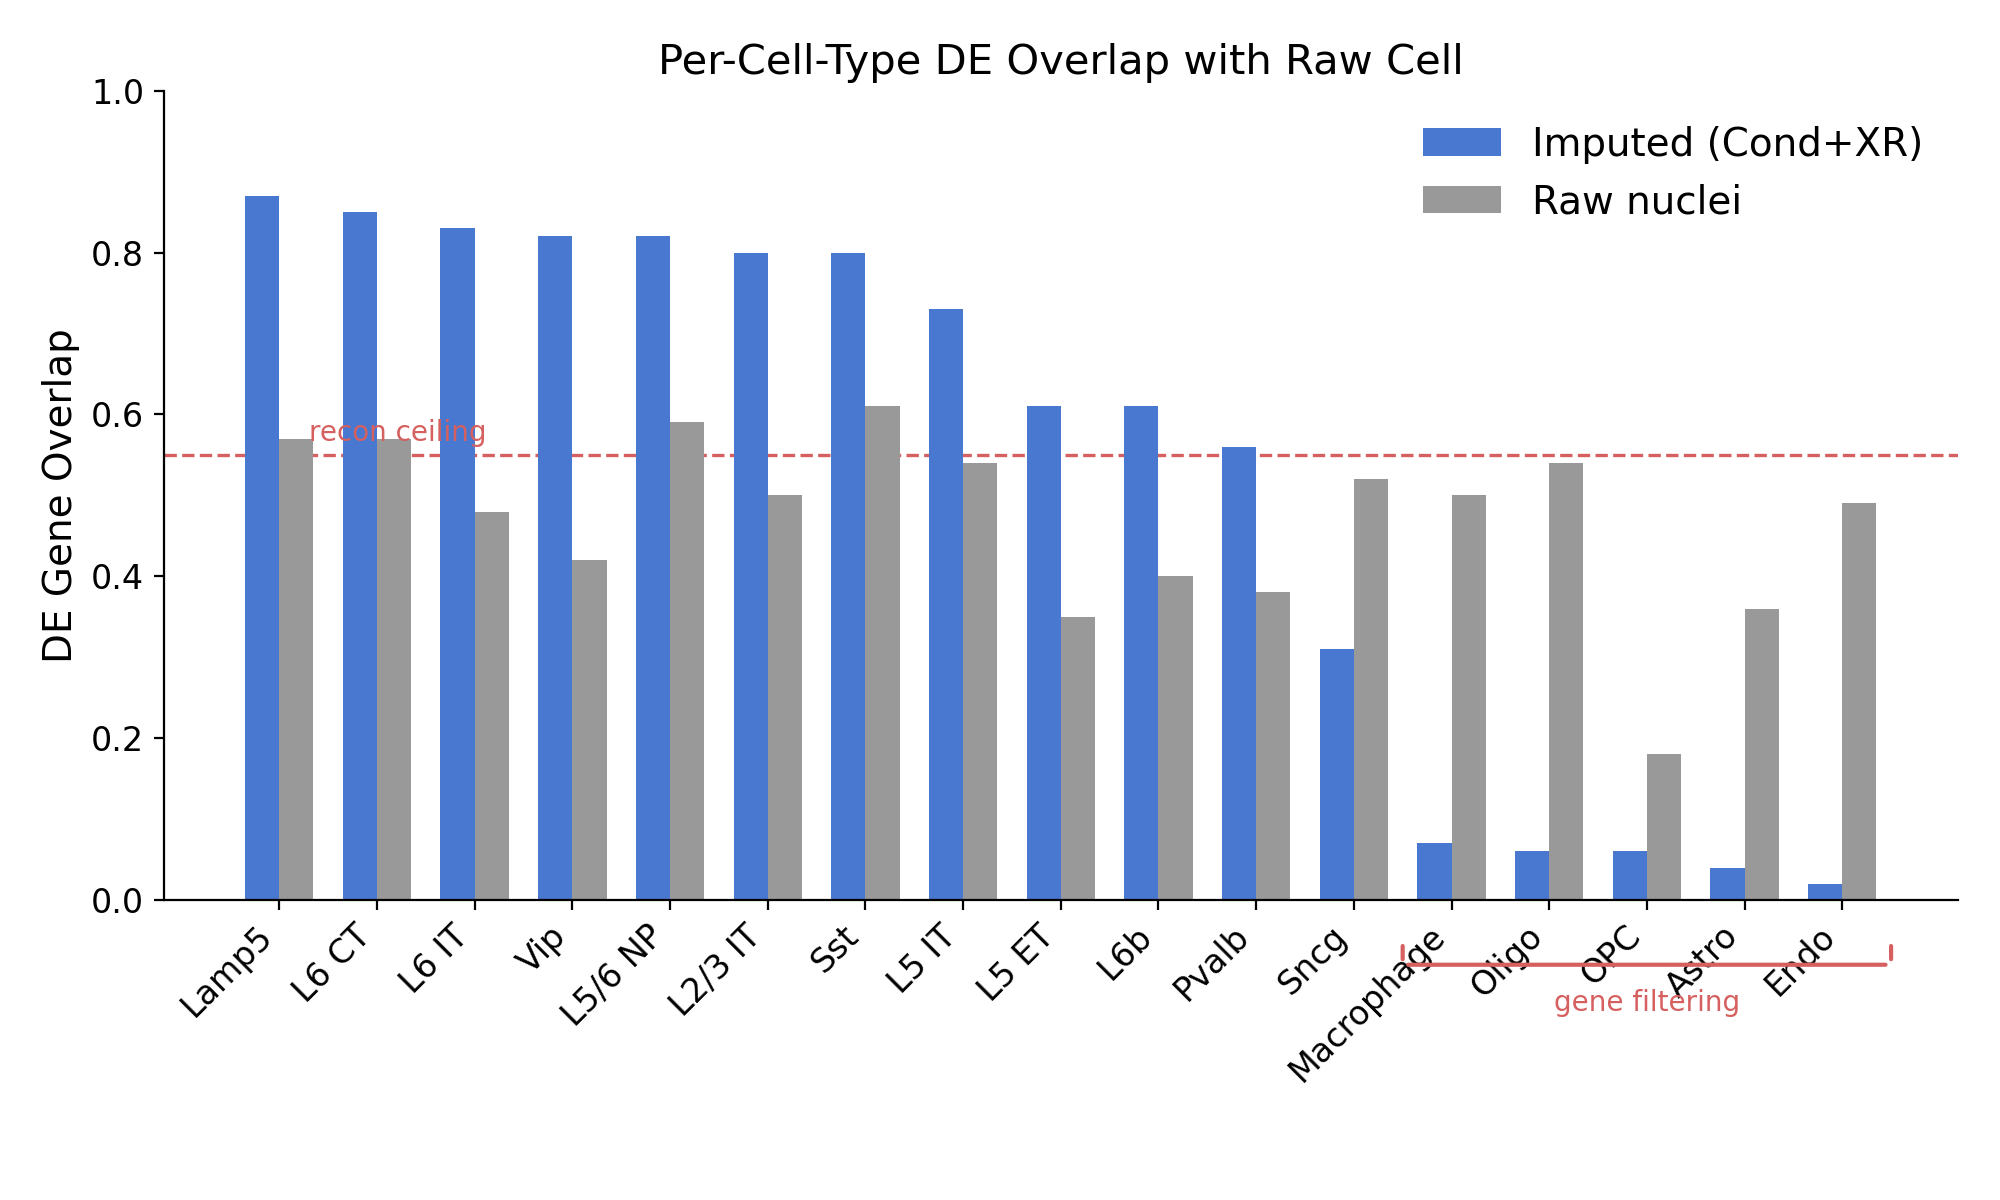
\includegraphics[width=\textwidth]{per_ct_de_overlap.png}
\end{column}
\end{columns}
\end{frame}

% ============================================================
% SLIDE 11: Gene stratification
% ============================================================
\begin{frame}{Imputation Quality Scales with Cell--Nucleus Divergence}
\centering
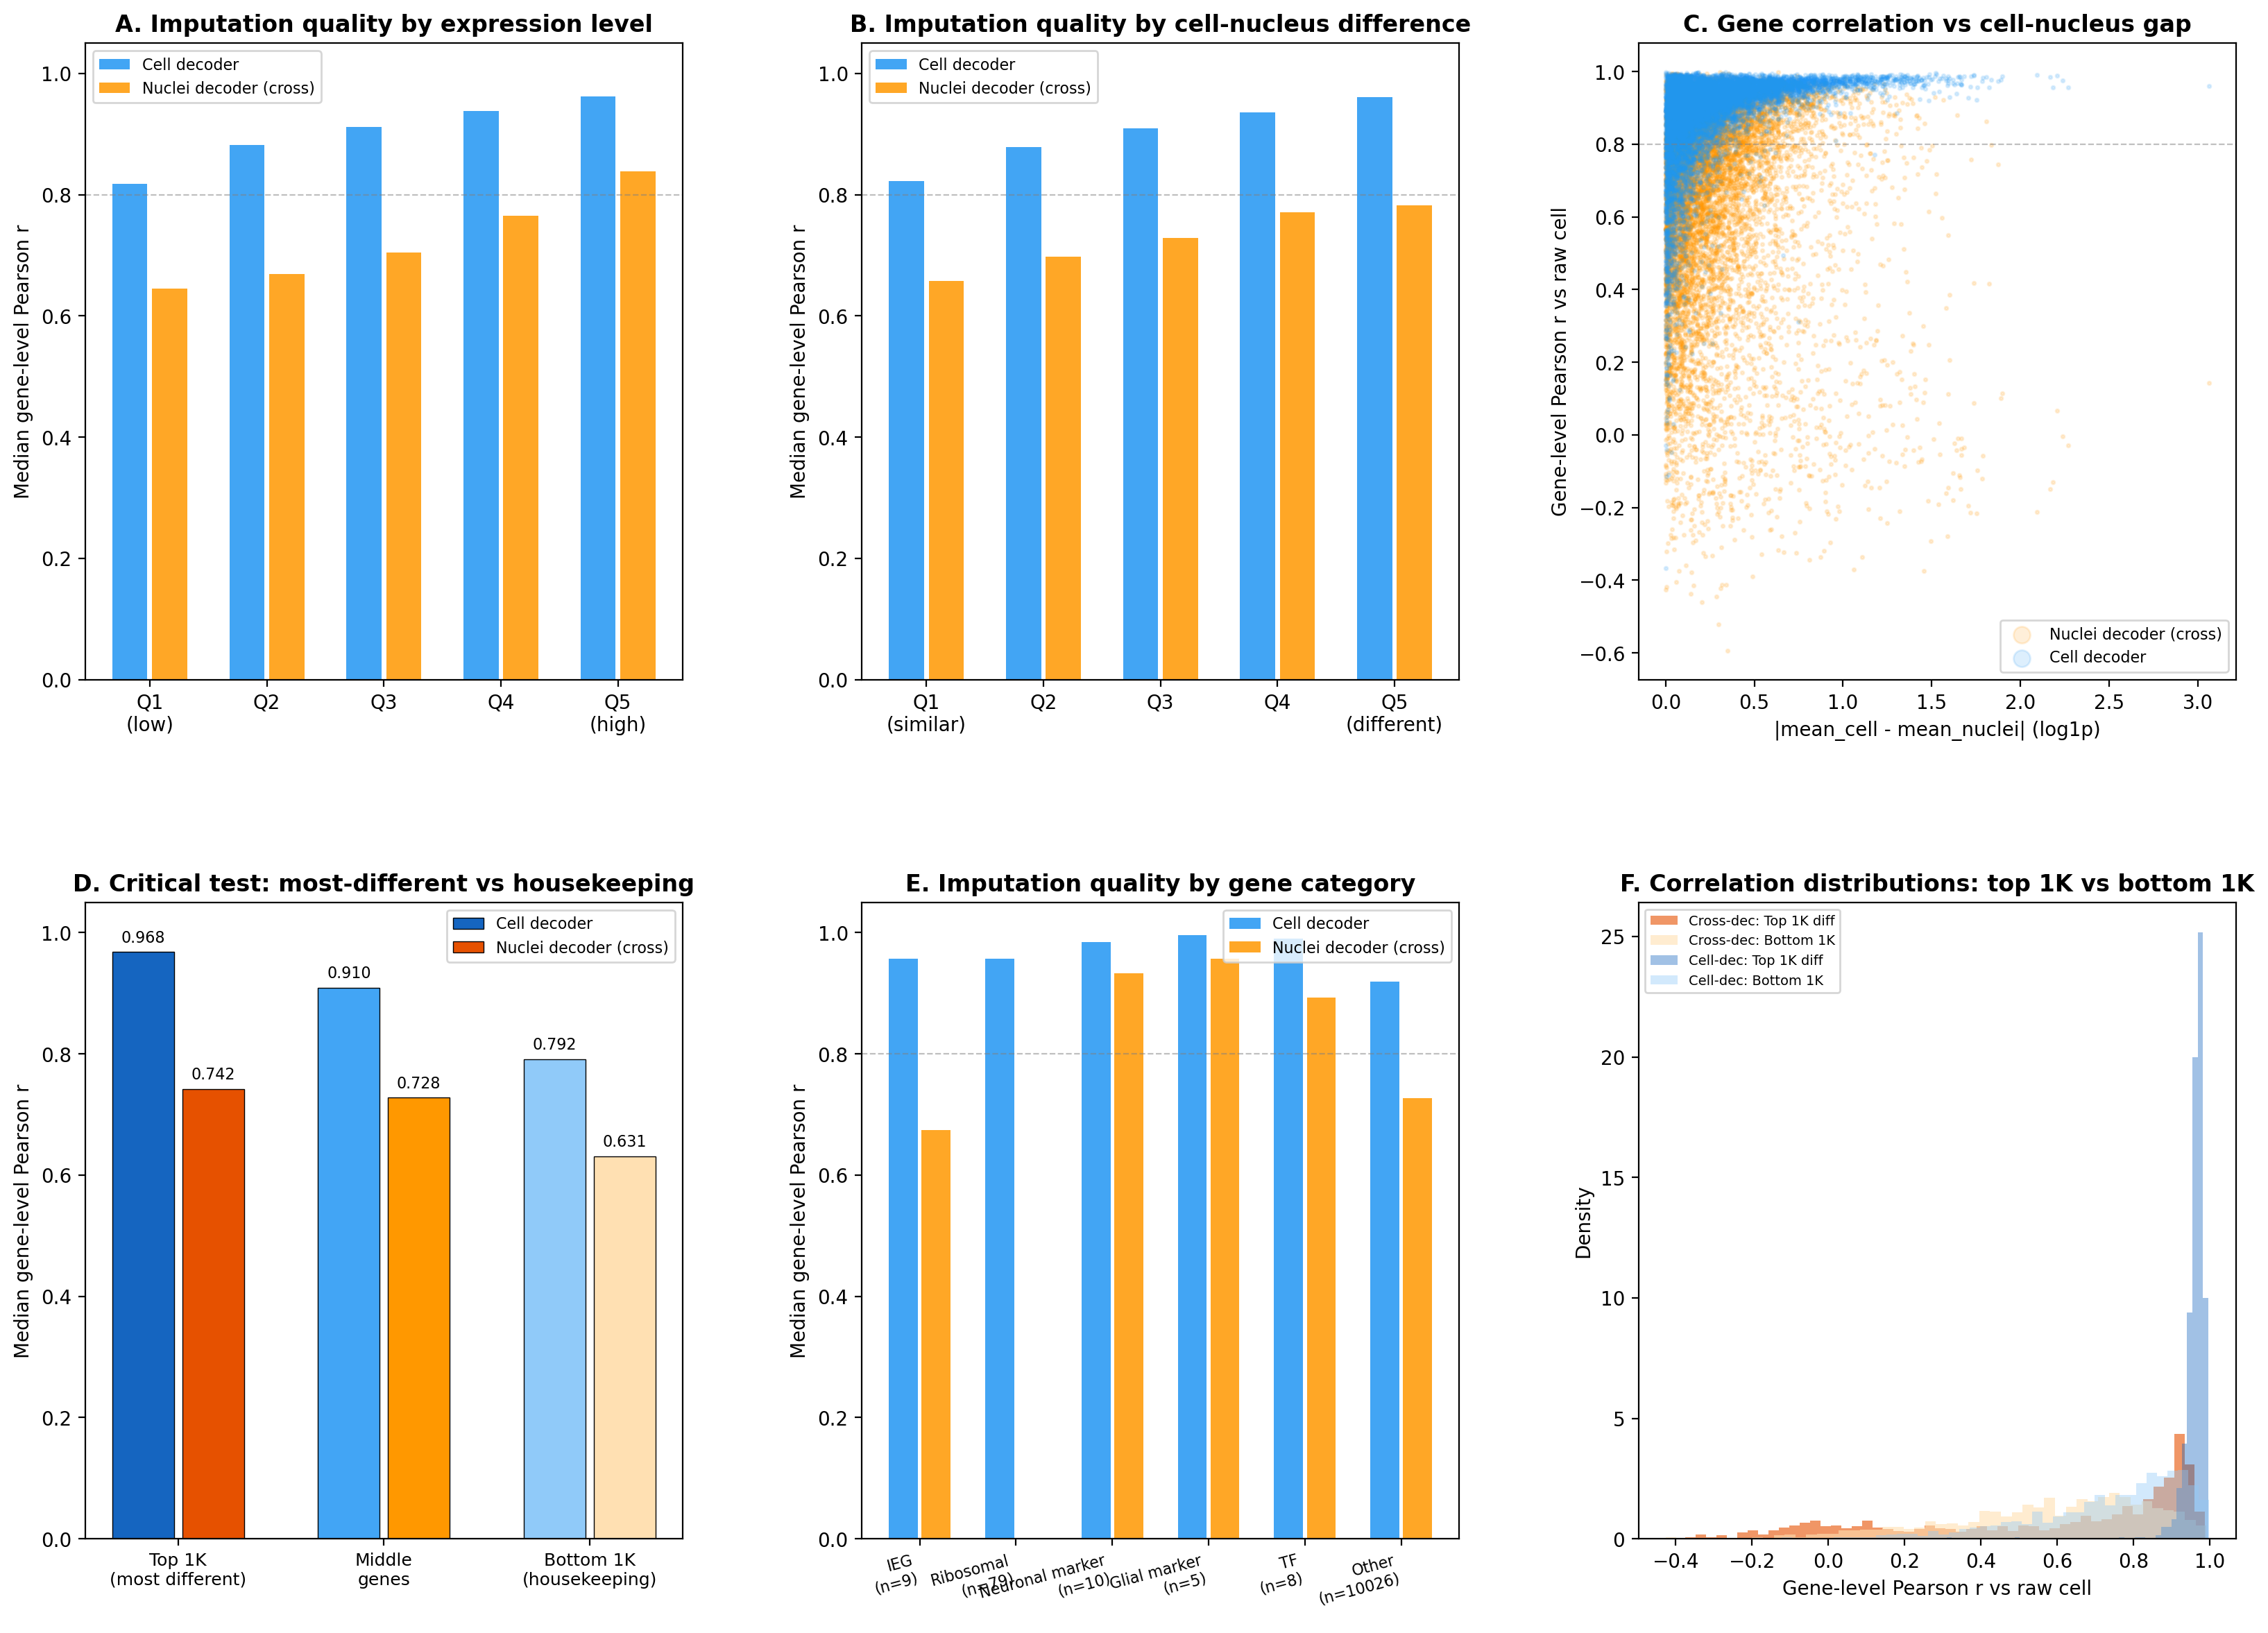
\includegraphics[width=0.88\textwidth, height=0.65\textheight, keepaspectratio]{gene_strat_overview.png}

\vspace{0.1em}
{\scriptsize Most-different genes (Q5): median $r = 0.83$, 55\% above $r > 0.8$. Cell-type markers $r > 0.99$.}
\end{frame}

% ============================================================
% SLIDE 11b: IEG detail (backup/optional)
% ============================================================
\begin{frame}{Marker Genes Excel; IEGs Remain the Frontier}
\centering
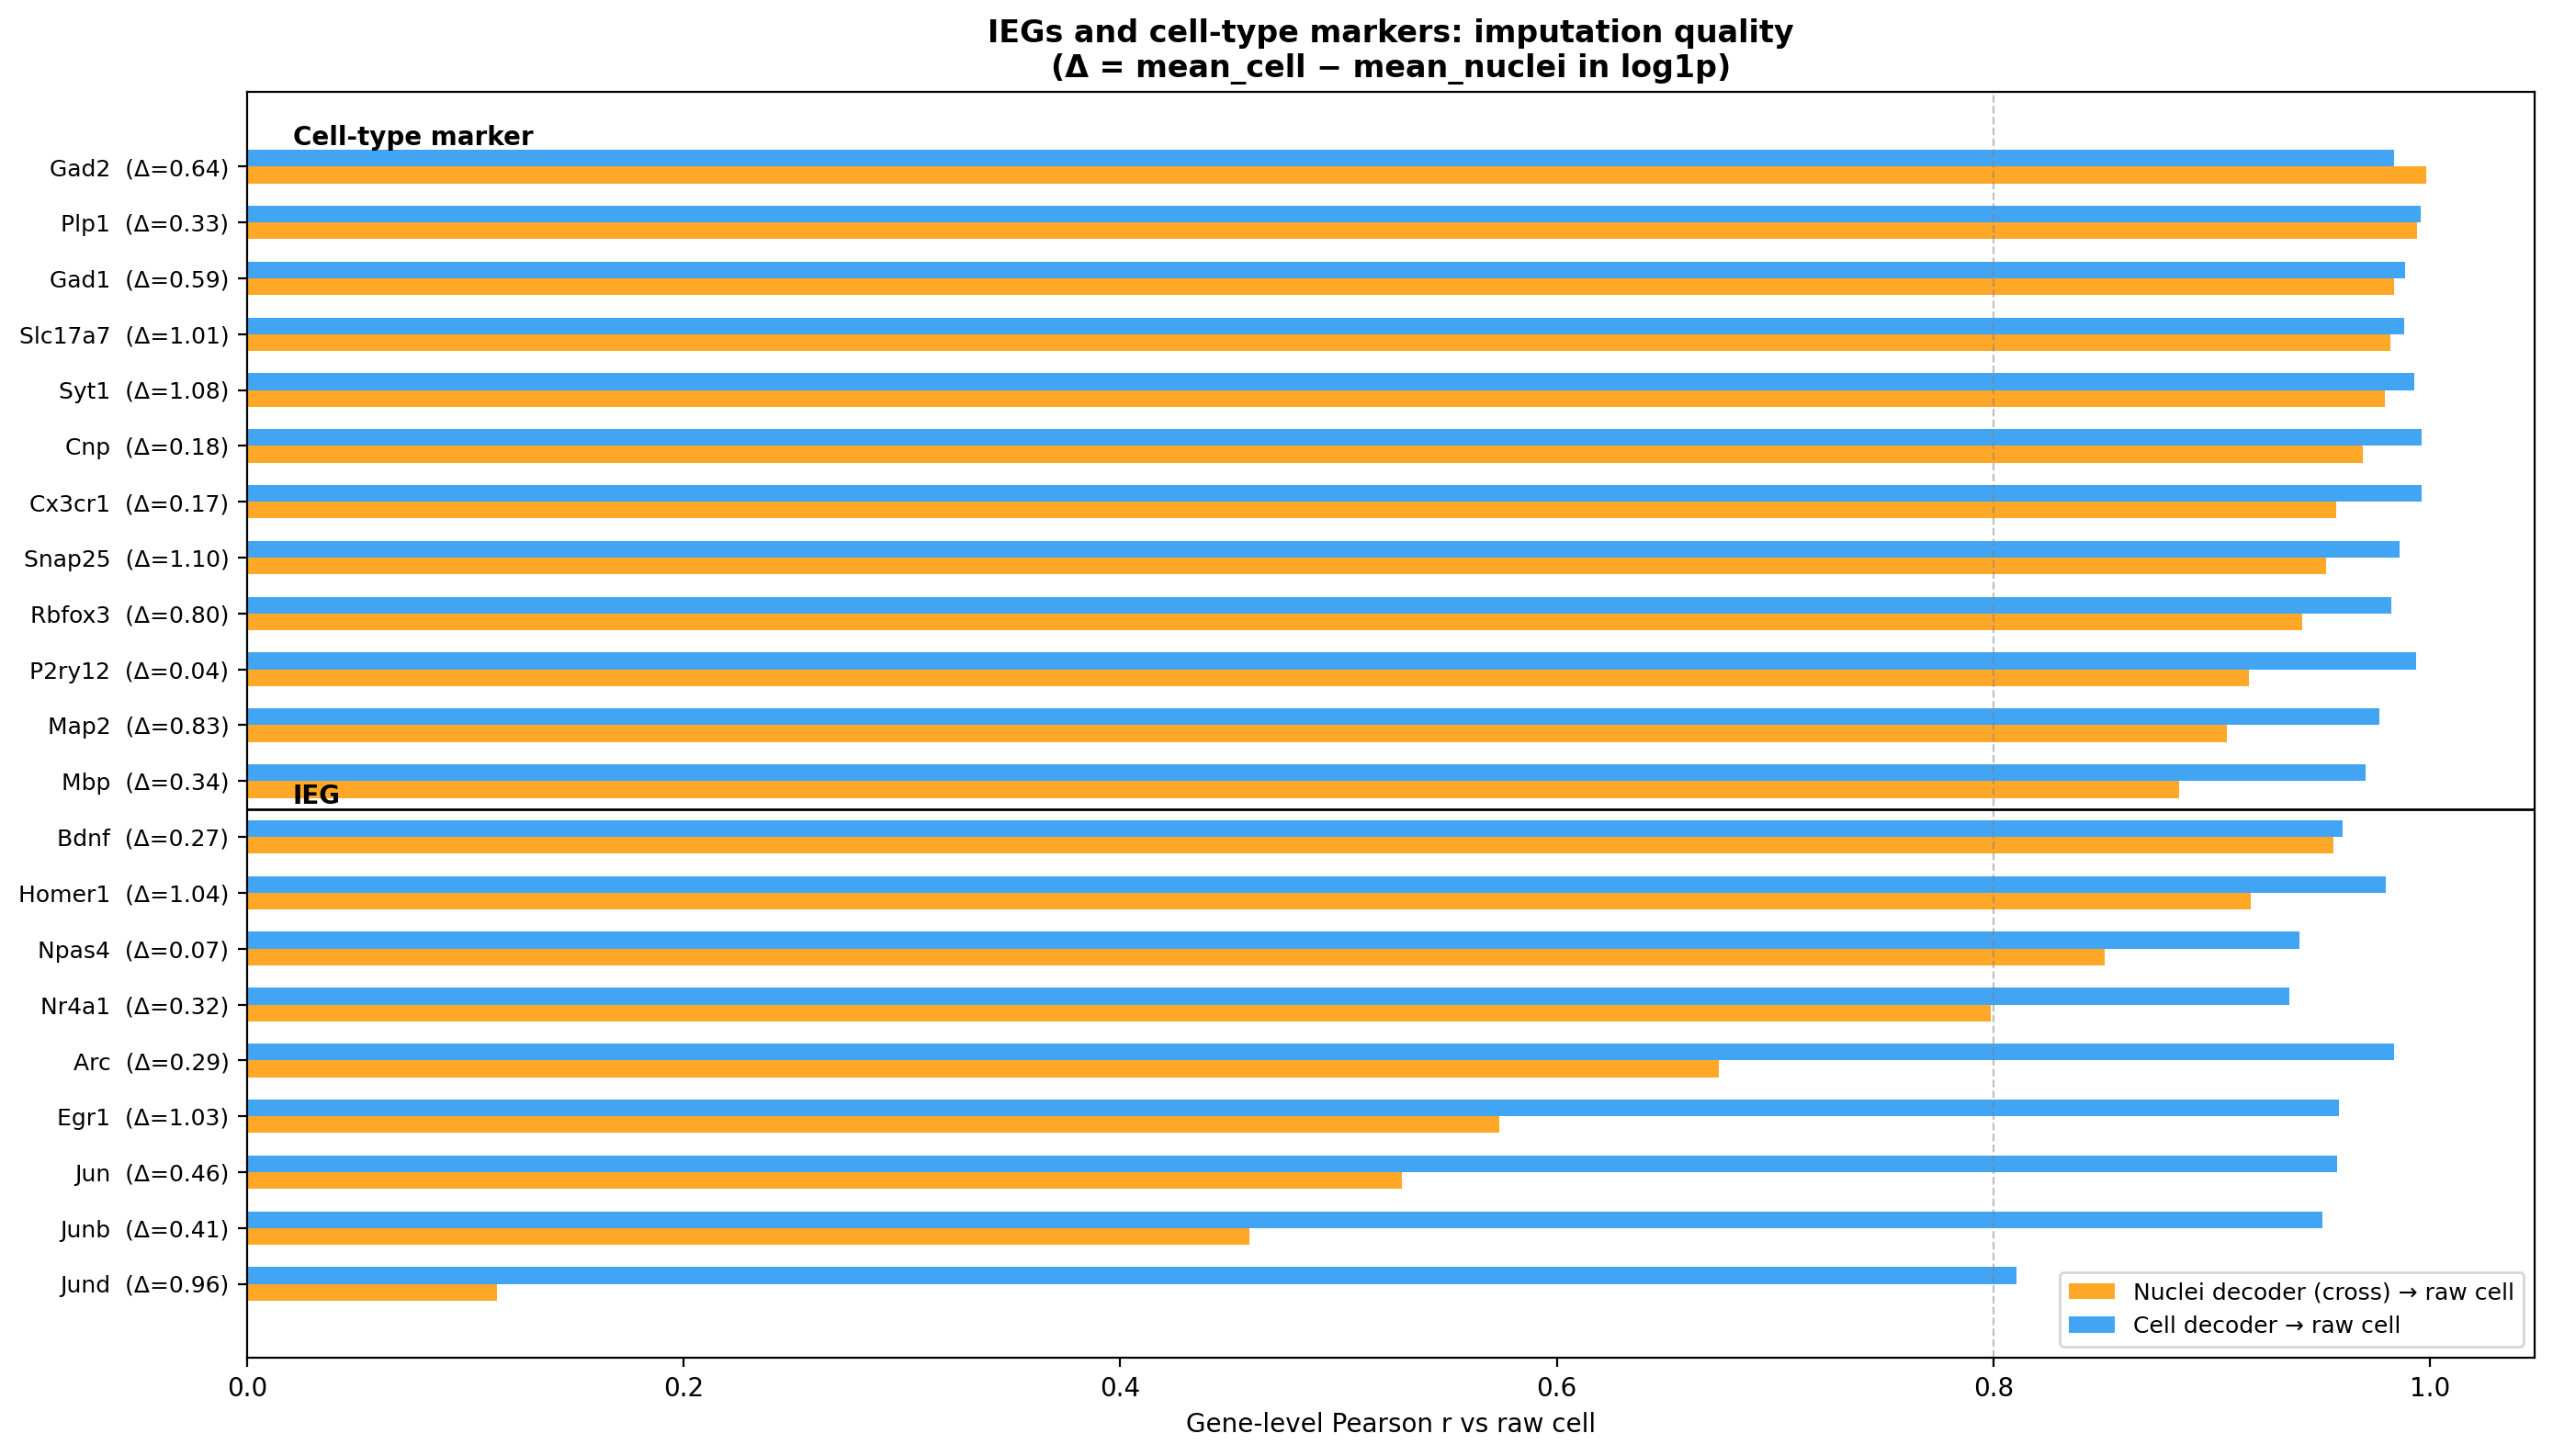
\includegraphics[width=0.82\textwidth, height=0.65\textheight, keepaspectratio]{ieg_marker_detail.png}

\vspace{0.1em}
{\scriptsize Gad2, Plp1, Slc17a7: $r > 0.99$. IEGs (Fos, Egr1, Jun): $r \approx 0.1$--$0.6$ --- hardest to impute.}
\end{frame}

% ============================================================
% SLIDE 12: Training dynamics
% ============================================================
\begin{frame}{Cross-Decode Quality Improves as Each Loss Activates}
\begin{columns}[c]
\begin{column}{0.48\textwidth}
\centering
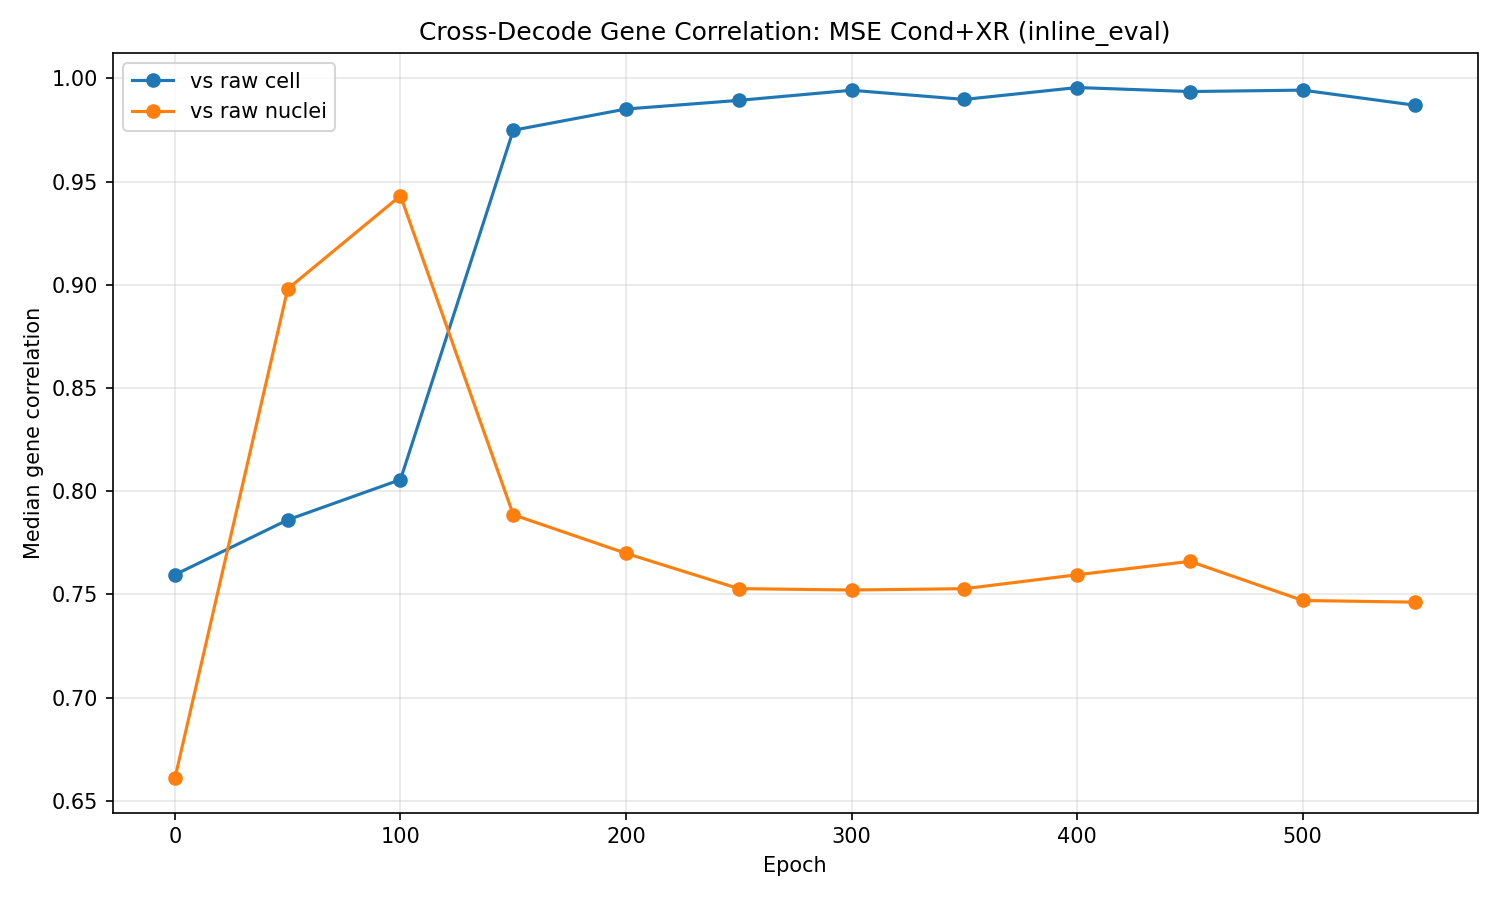
\includegraphics[width=\textwidth]{cross_dec_corr_time.png}
\end{column}
\begin{column}{0.48\textwidth}
\centering
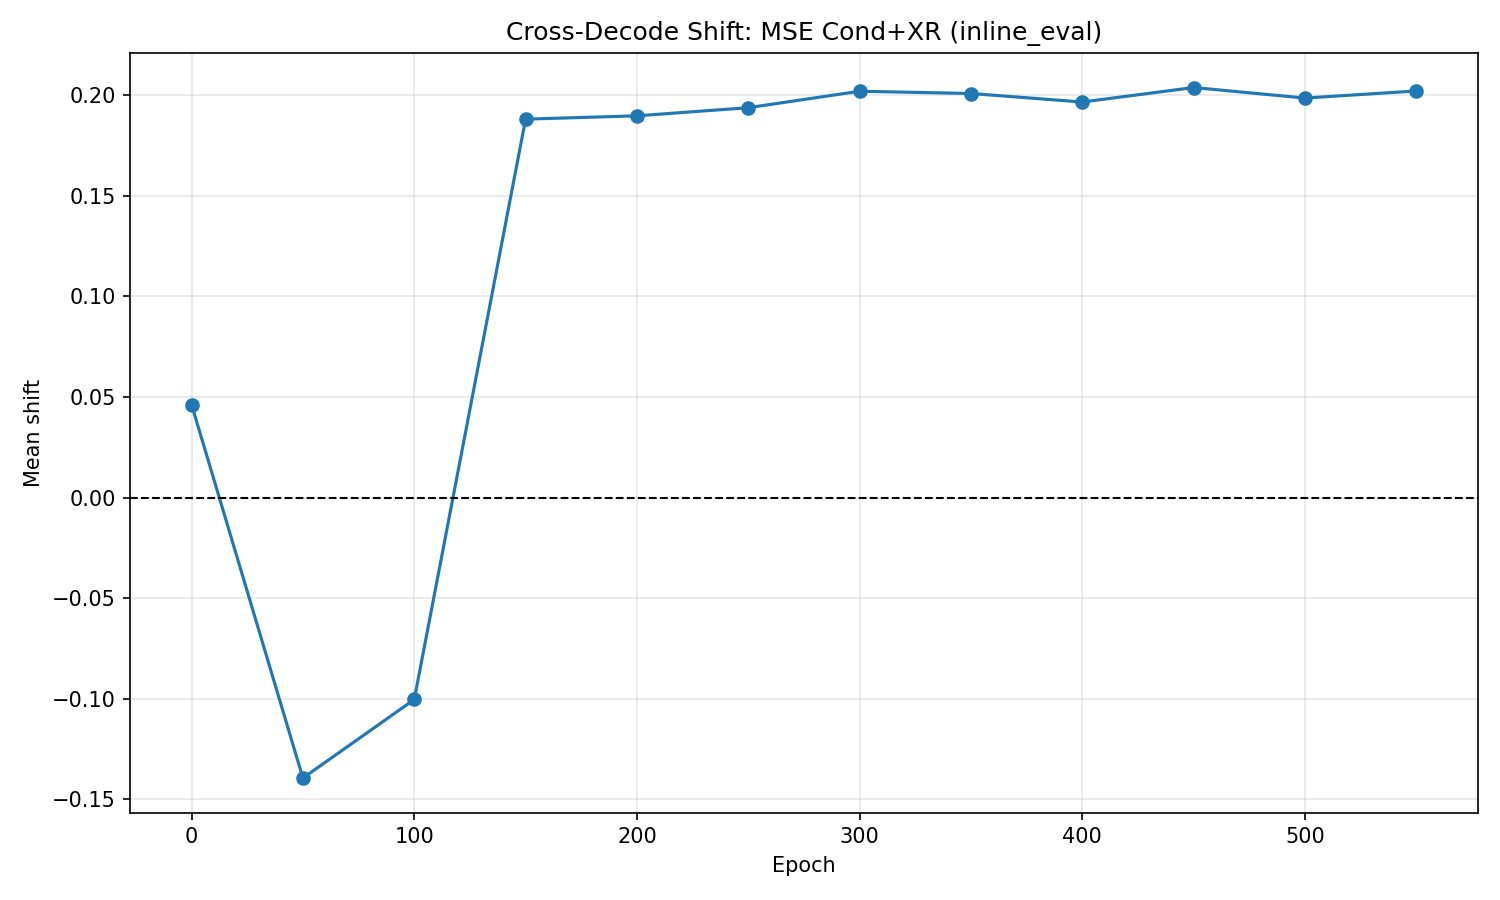
\includegraphics[width=\textwidth]{cross_dec_shift_time.png}
\end{column}
\end{columns}

\vspace{0.3em}
{\small Cross-recons onset (epoch 100) drives the largest quality jump. Metrics stable by epoch 400.}
\end{frame}

% ============================================================
% SLIDE 13: UMAPs
% ============================================================
\begin{frame}{UMAPs Confirm Alignment and Cross-Decode Quality}
\begin{columns}[c]
\begin{column}{0.32\textwidth}
\centering
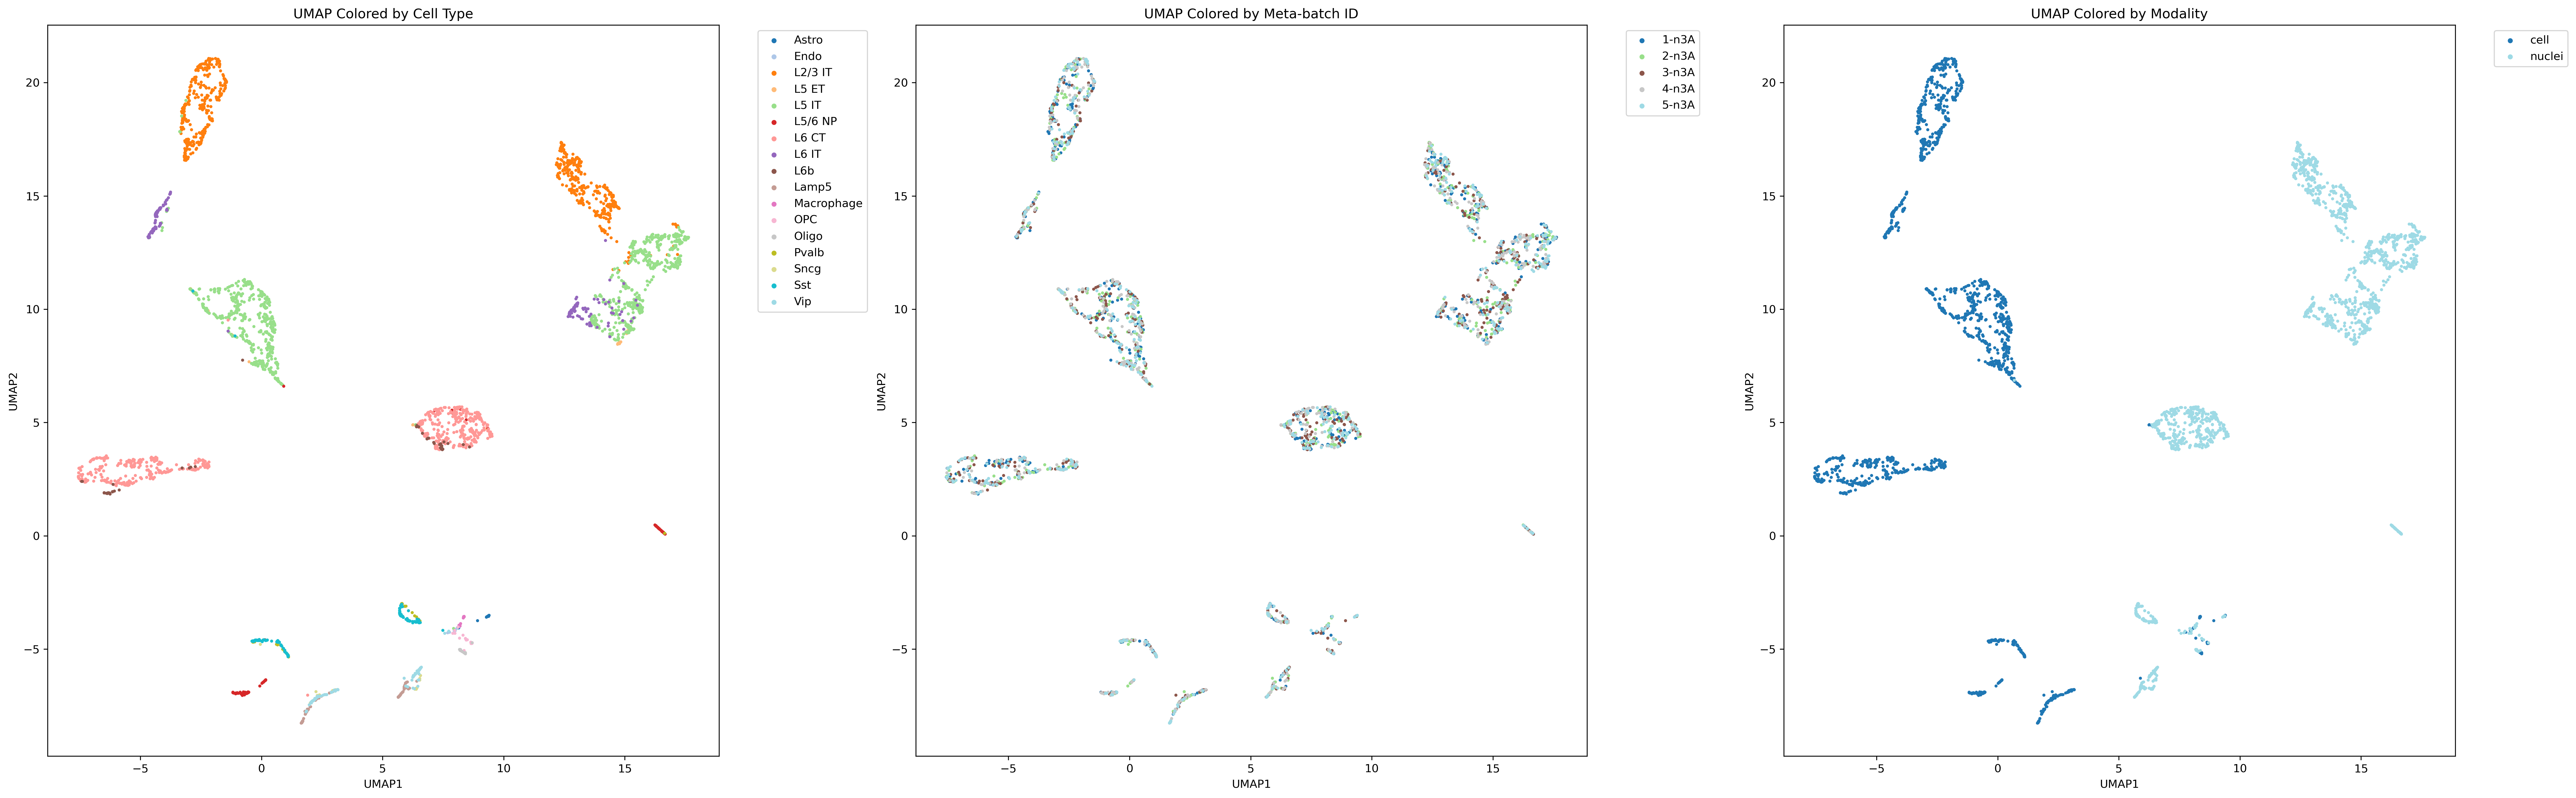
\includegraphics[width=\textwidth]{umap_e0_encoded.png}\\
{\scriptsize Epoch 0 --- encoded}
\end{column}
\begin{column}{0.32\textwidth}
\centering
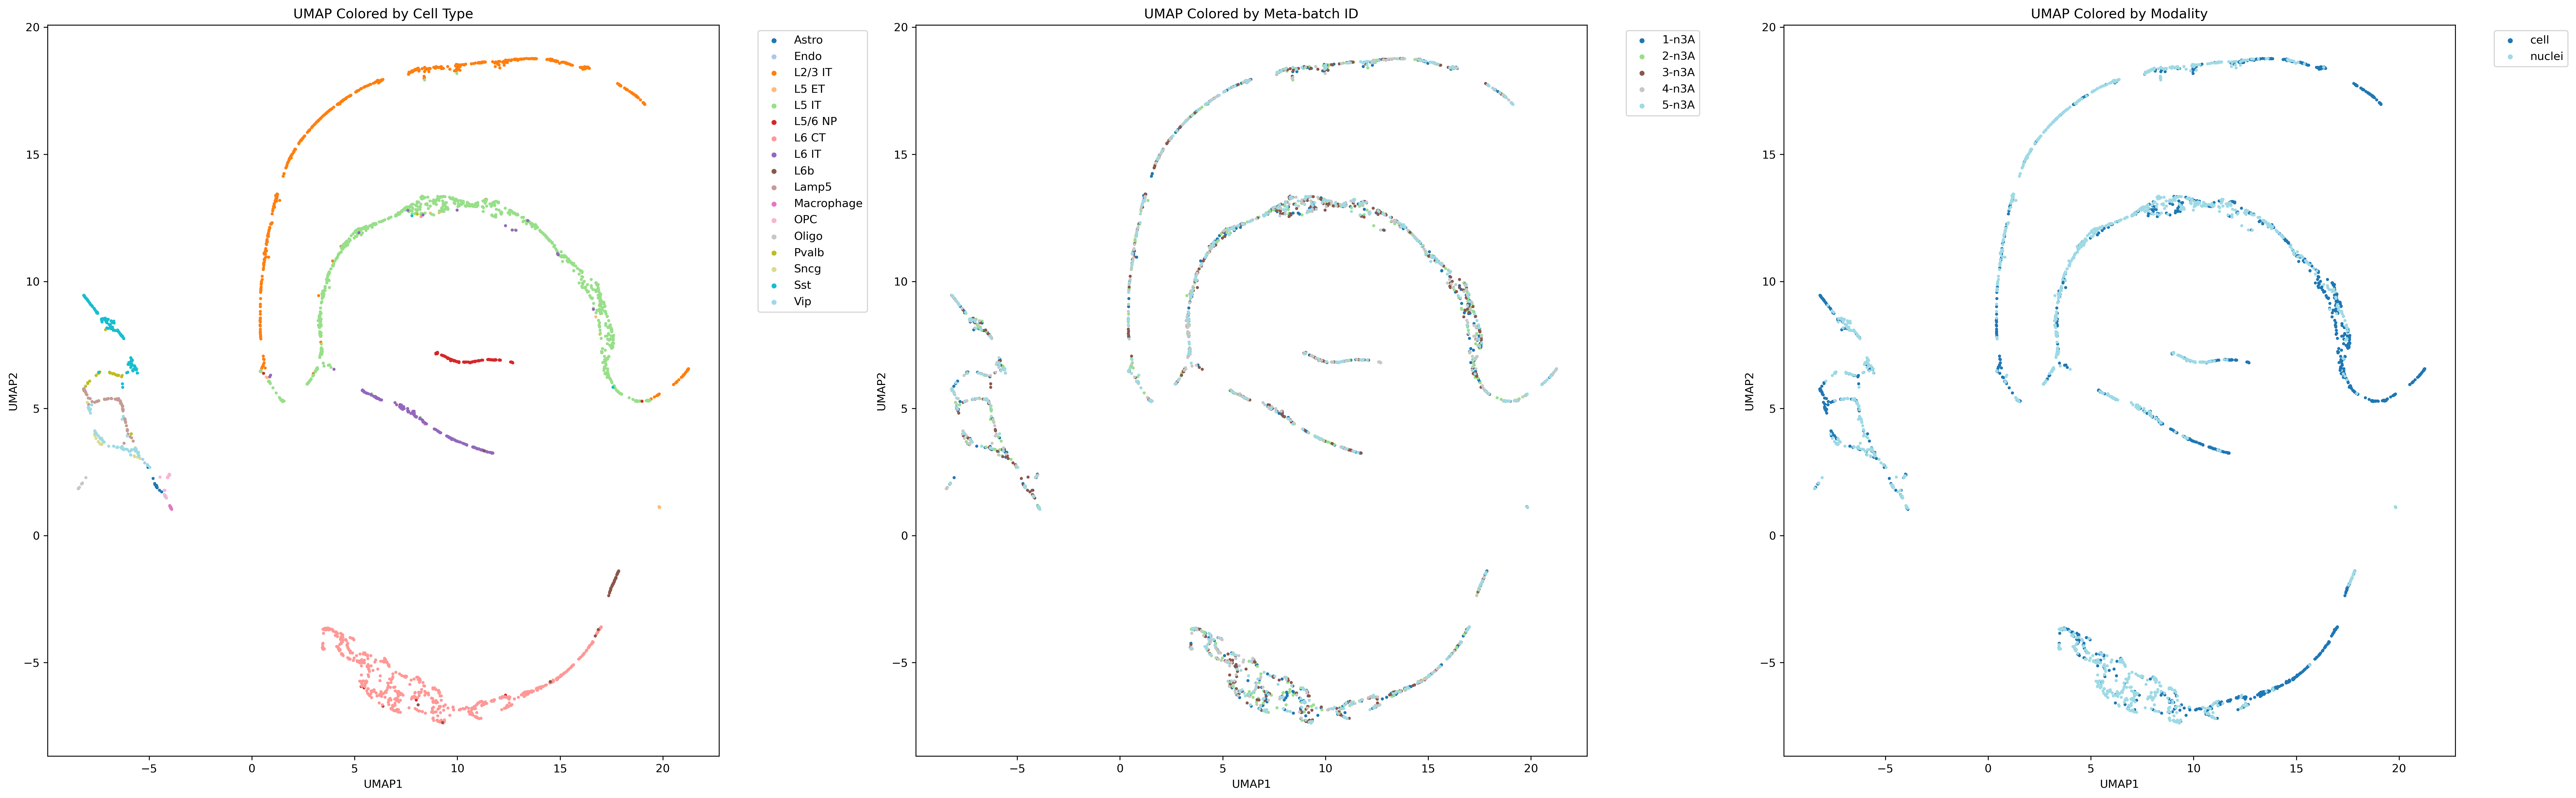
\includegraphics[width=\textwidth]{umap_e599_encoded.png}\\
{\scriptsize Epoch 599 --- encoded}
\end{column}
\begin{column}{0.32\textwidth}
\centering
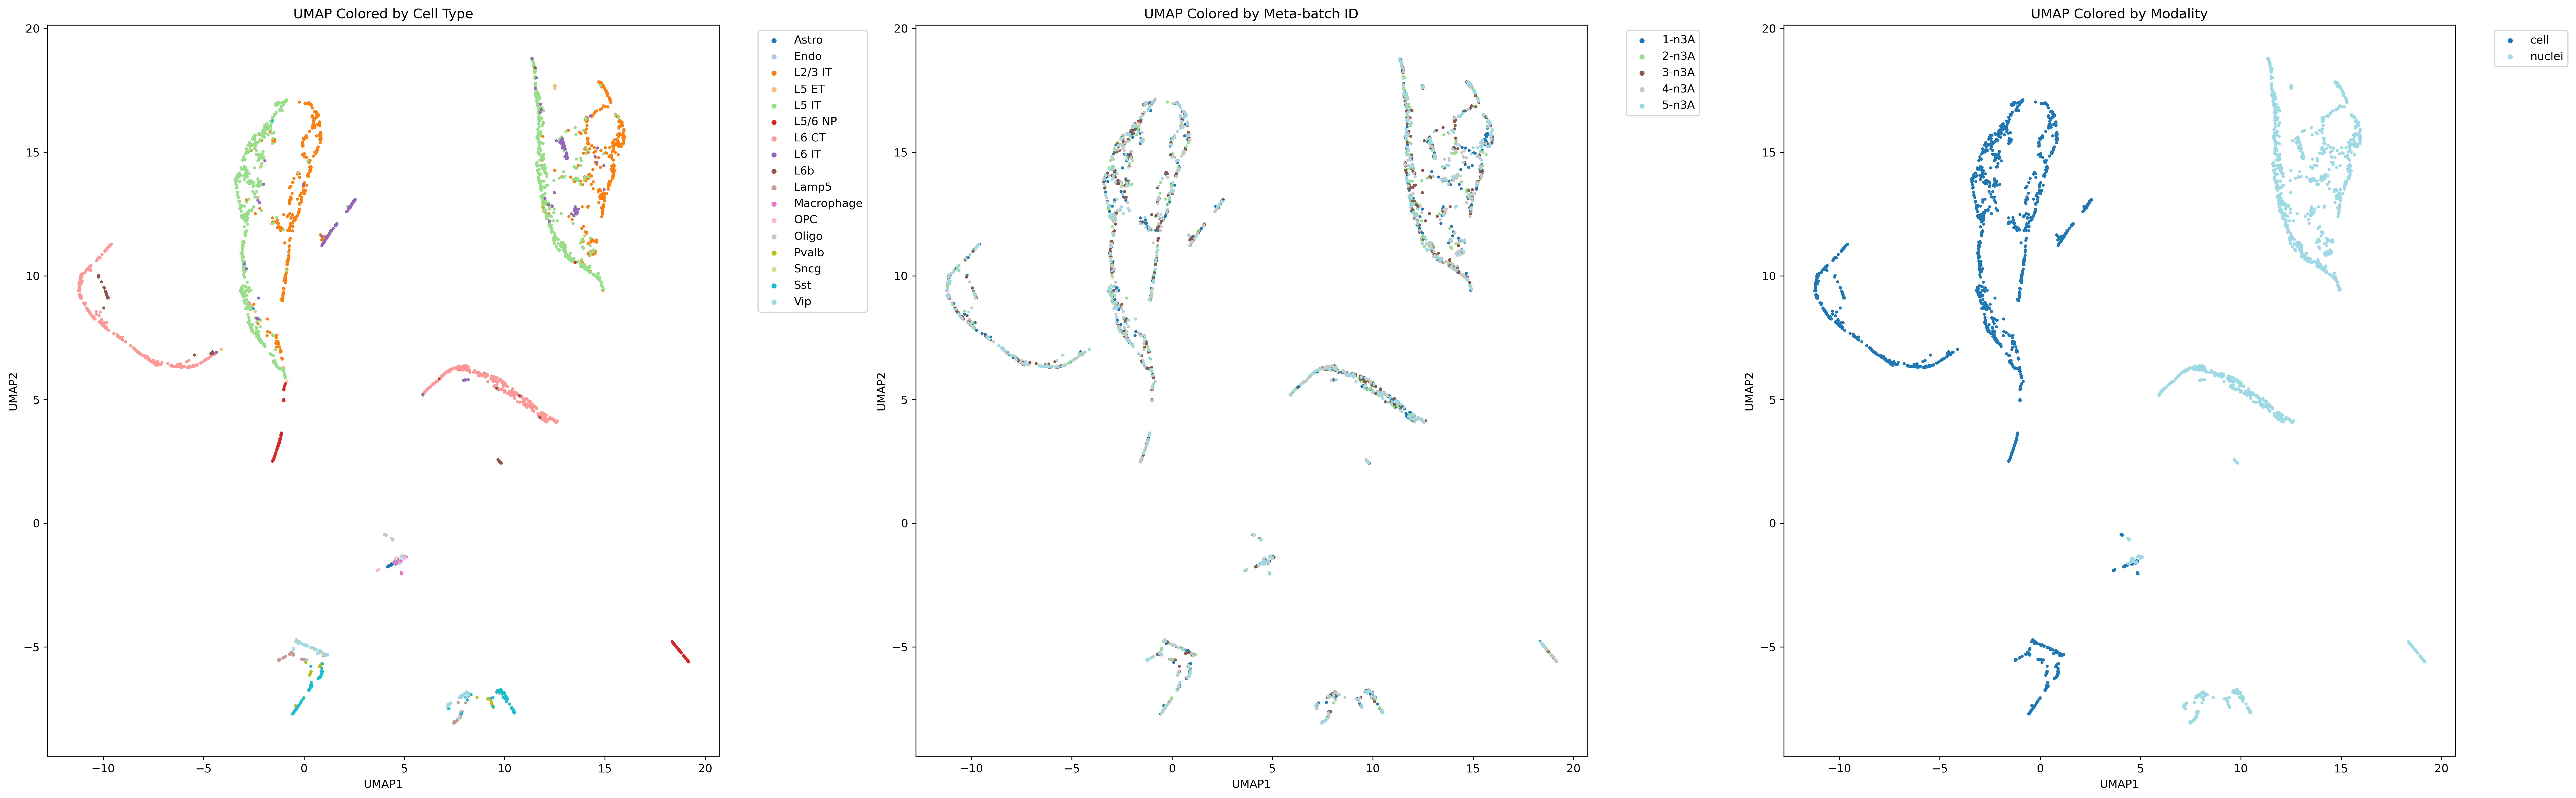
\includegraphics[width=\textwidth]{umap_e599_decoded.png}\\
{\scriptsize Epoch 599 --- decoded}
\end{column}
\end{columns}

\vspace{0.3em}
{\small Cell types cluster cleanly. Modalities overlap after training. Cross-decoded output is cell-like.}
\end{frame}

% ============================================================
% SECTION 4: HONEST ASSESSMENT
% ============================================================
\section{How Good Is It Really?}

% ============================================================
% SLIDE 14: Reconstruction ceiling
% ============================================================
\begin{frame}{Cross-Modal Translation Nearly Matches Reconstruction Ceiling}
\begin{columns}[T]
\begin{column}{0.40\textwidth}
\begin{itemize}
    \item Cell recon: $r{=}0.84$, classif 93\%, DE 0.55
    \item Cross-decode: classif \textbf{96\%}, DE 0.52
    \item Gap is $<$3\% --- translation is nearly lossless
\end{itemize}
\end{column}
\begin{column}{0.58\textwidth}
\centering
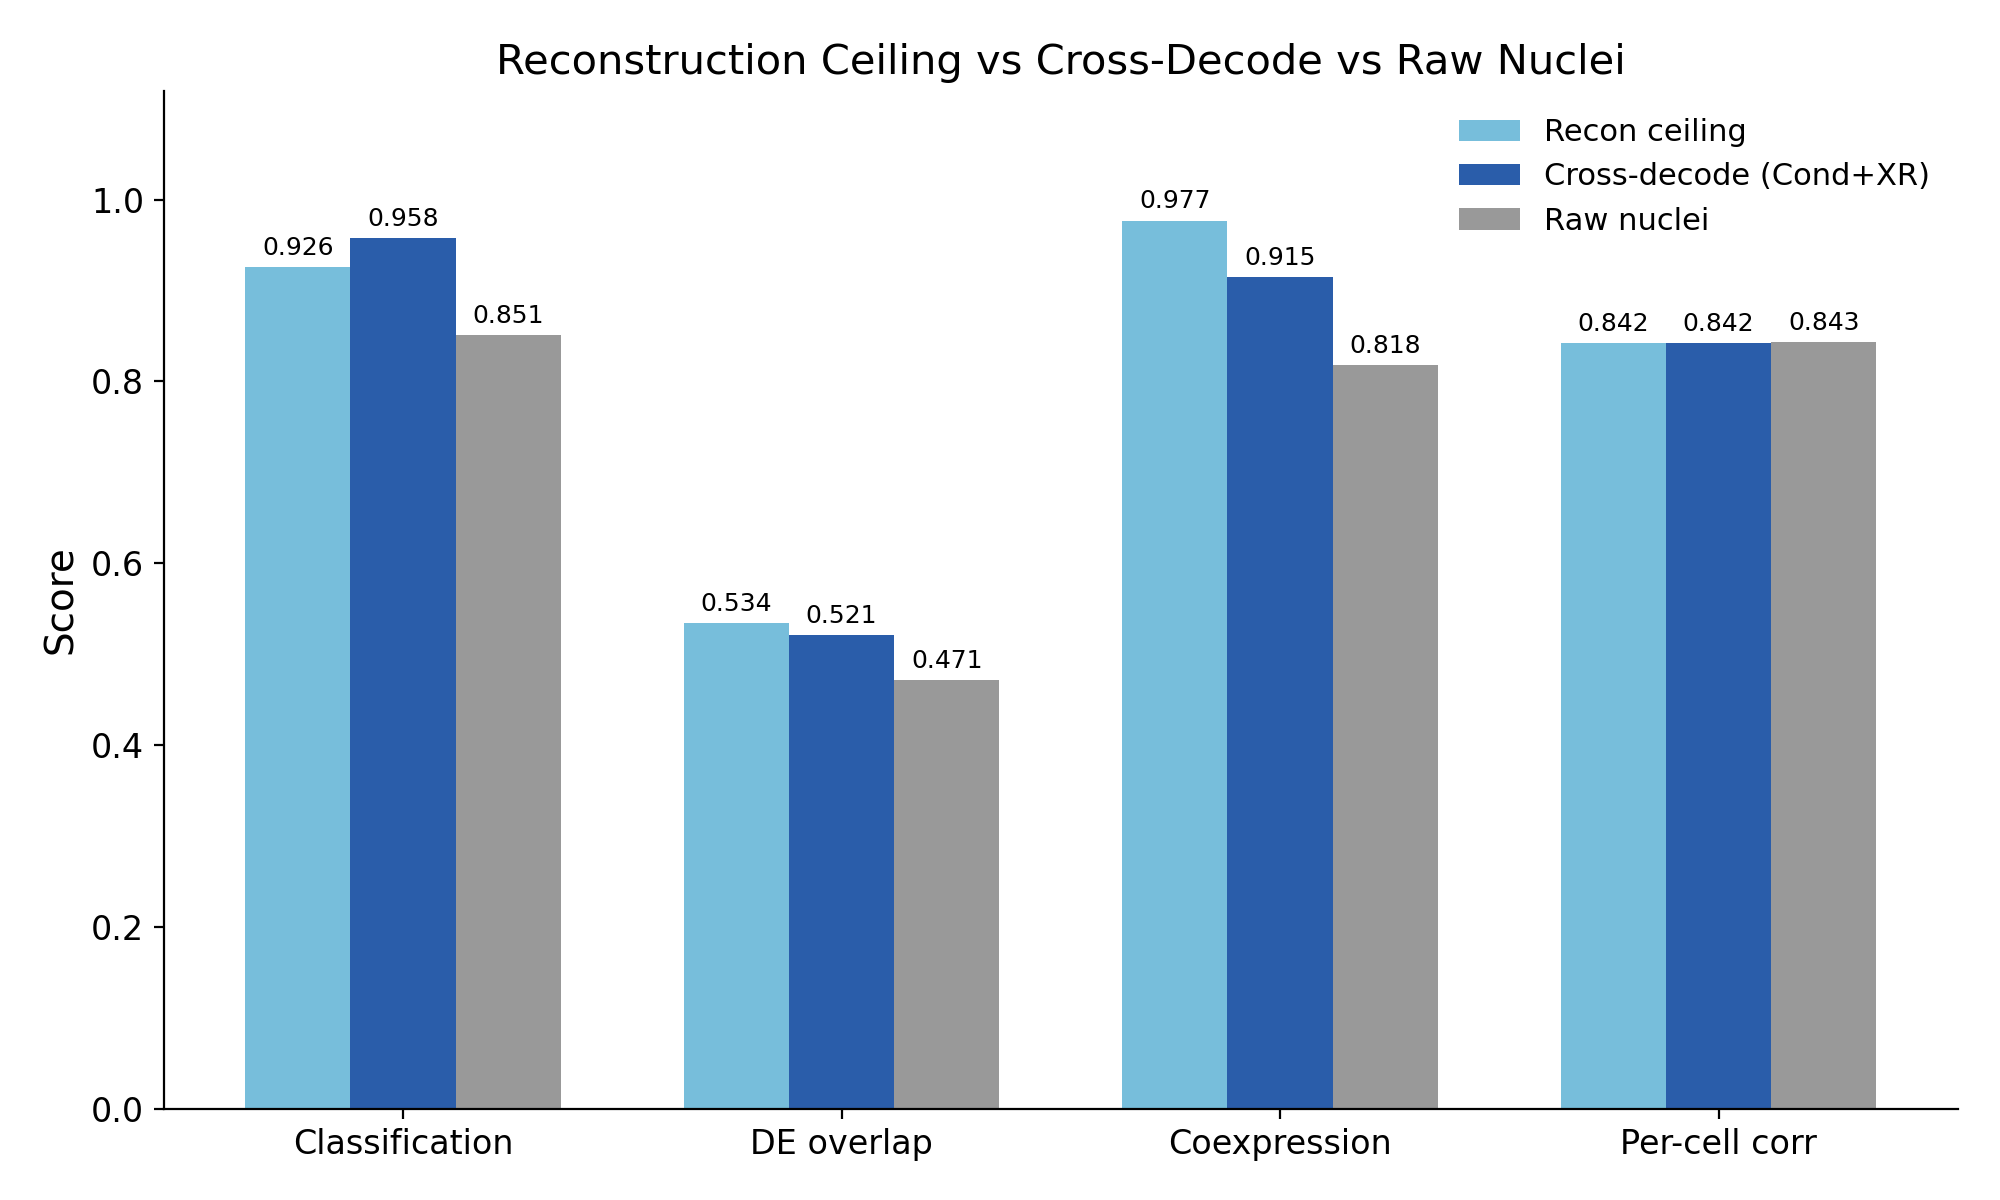
\includegraphics[width=\textwidth]{recon_ceiling_comparison.png}
\end{column}
\end{columns}
\end{frame}

% ============================================================
% SLIDE 15: Variance / honest
% ============================================================
\begin{frame}{Per-Cell Variance Is a General VAE Bottleneck}
\begin{columns}[T]
\begin{column}{0.42\textwidth}
\begin{itemize}
    \item Recon retains $\sim$24\% of within-CT cell variance
    \item Cross-decode retains $\sim$8\% --- further loss, but not unique to cross-modal
    \item $z$ ablation: CT mean $z$ changes output $<$1\%
\end{itemize}

\vspace{0.5em}
{\small\textbf{Still useful}: classification, DE, coexpression are all cell-type--level analyses.}
\end{column}
\begin{column}{0.56\textwidth}
\centering
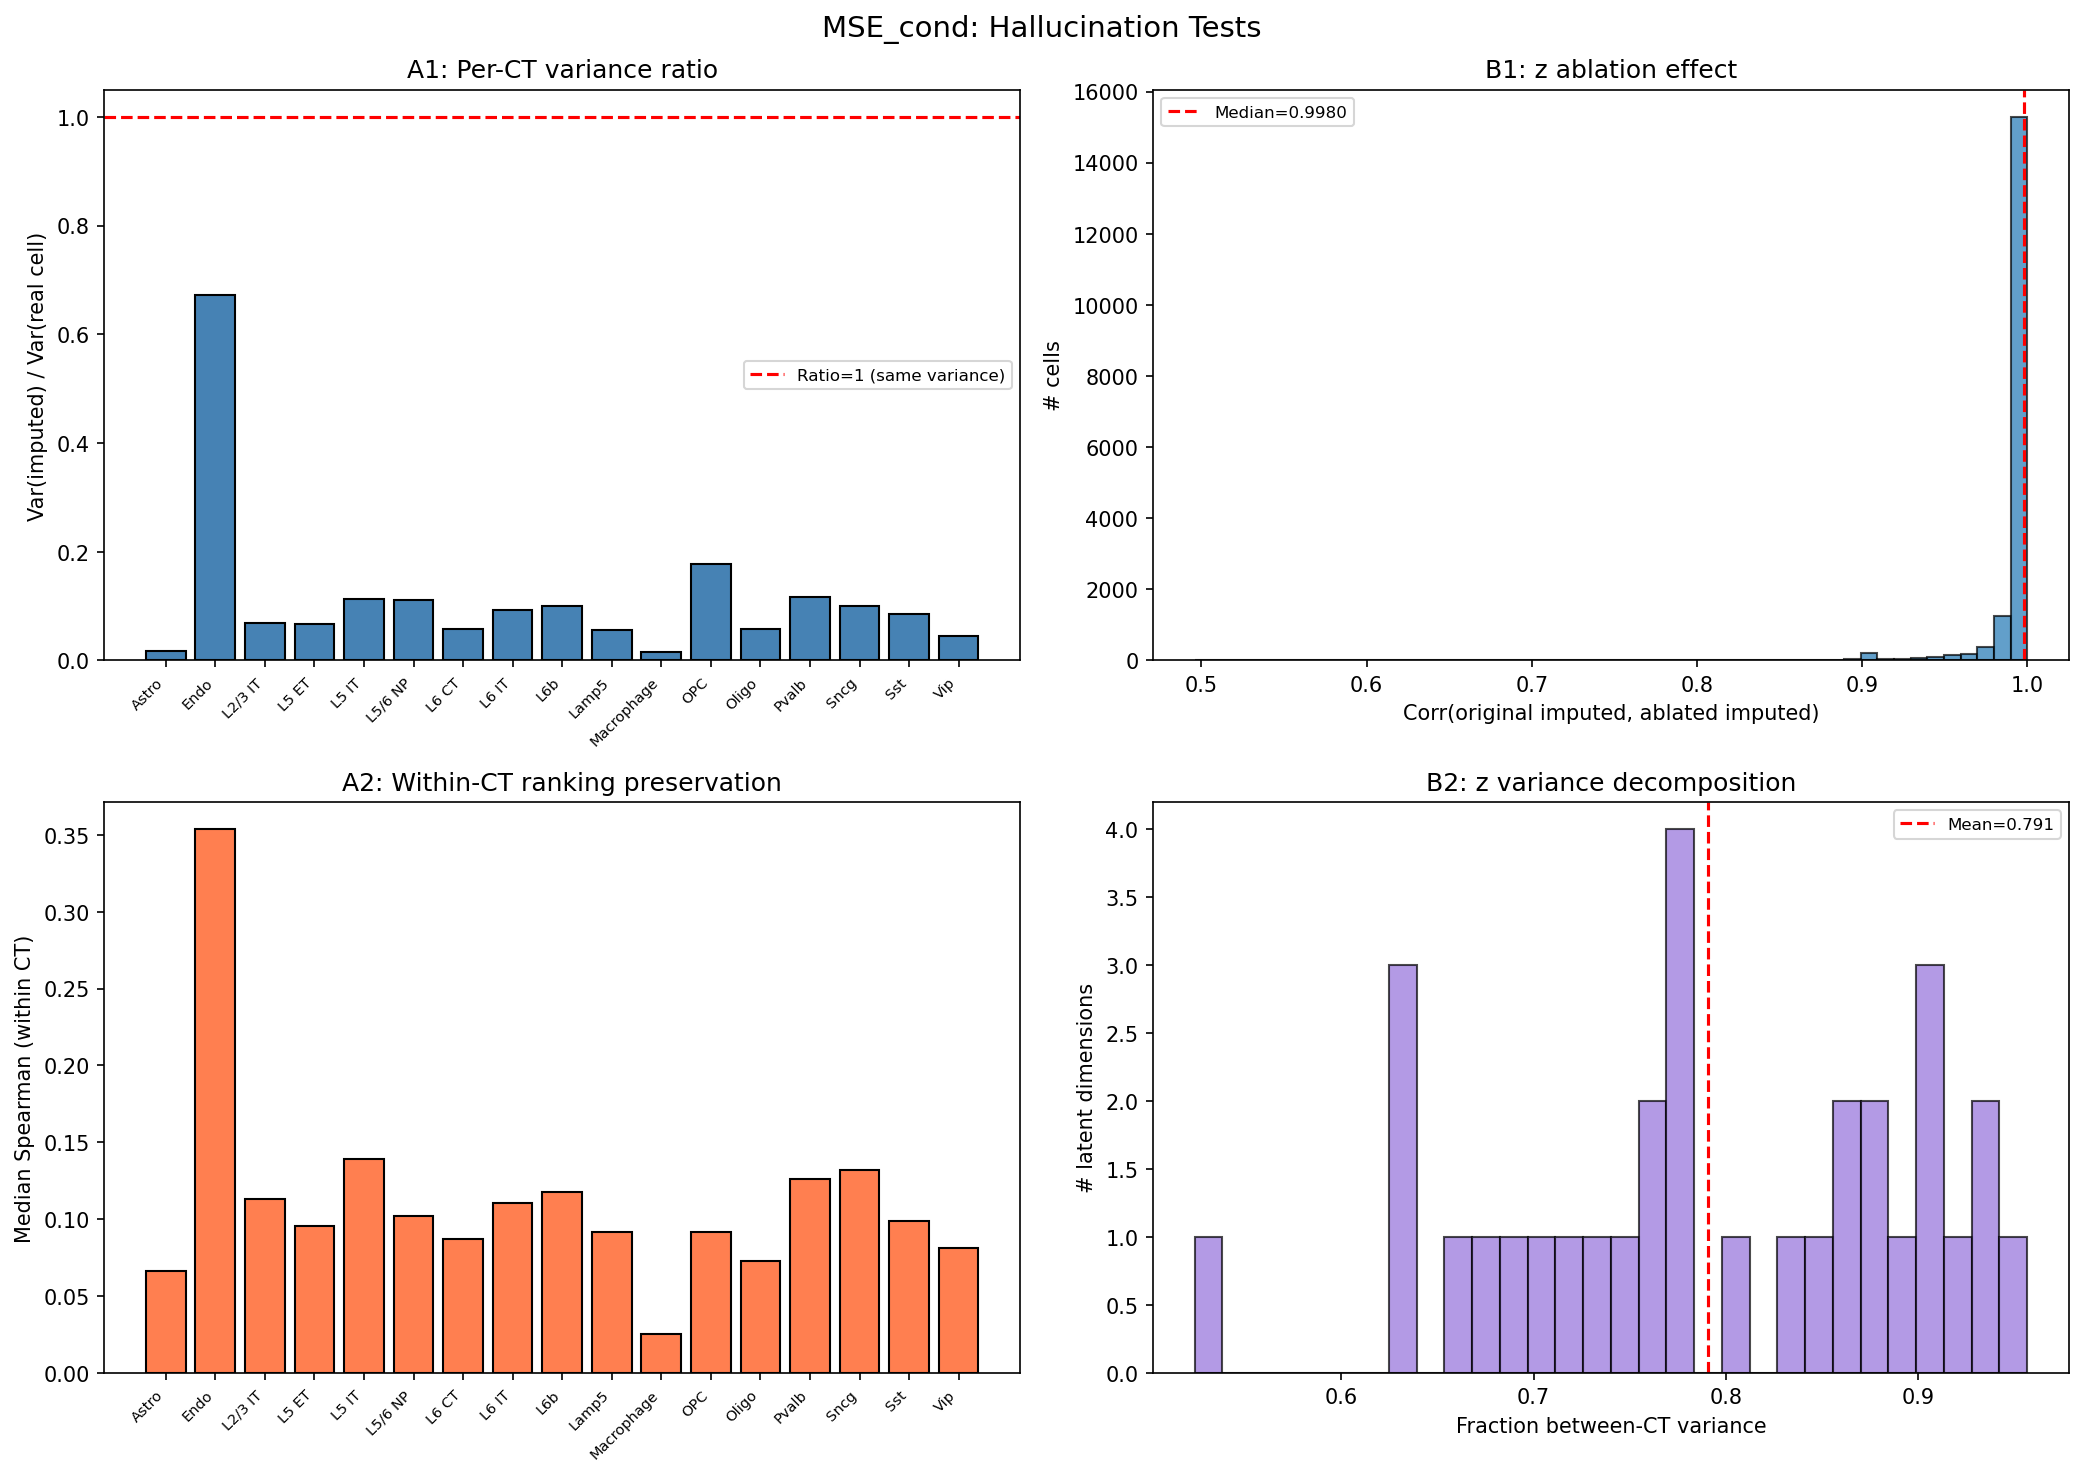
\includegraphics[width=\textwidth]{hallucination_cond.png}
\end{column}
\end{columns}
\end{frame}

% ============================================================
% SECTION 5: GENE FILTERING
% ============================================================
\section{Gene Filtering Fix}

% ============================================================
% SLIDE 16: Gene filtering problem
% ============================================================
\begin{frame}{5\% Global Filtering Drops 29 of 59 Cell-Type Markers}
\begin{columns}[T]
\begin{column}{0.42\textwidth}
\begin{itemize}
    \item Config B (10,134 genes) removes Aqp4, Mog, Pdgfra, Flt1, C1qa\ldots
    \item Rare types ($\sim$1--5\% of cells) fail global threshold
    \item Explains near-zero DE for non-neuronal types
\end{itemize}

\vspace{0.3em}
{\small Confirmed: same-modality recon also has Astro DE = 0.07 --- gene filtering, not model.}
\end{column}
\begin{column}{0.56\textwidth}
\centering
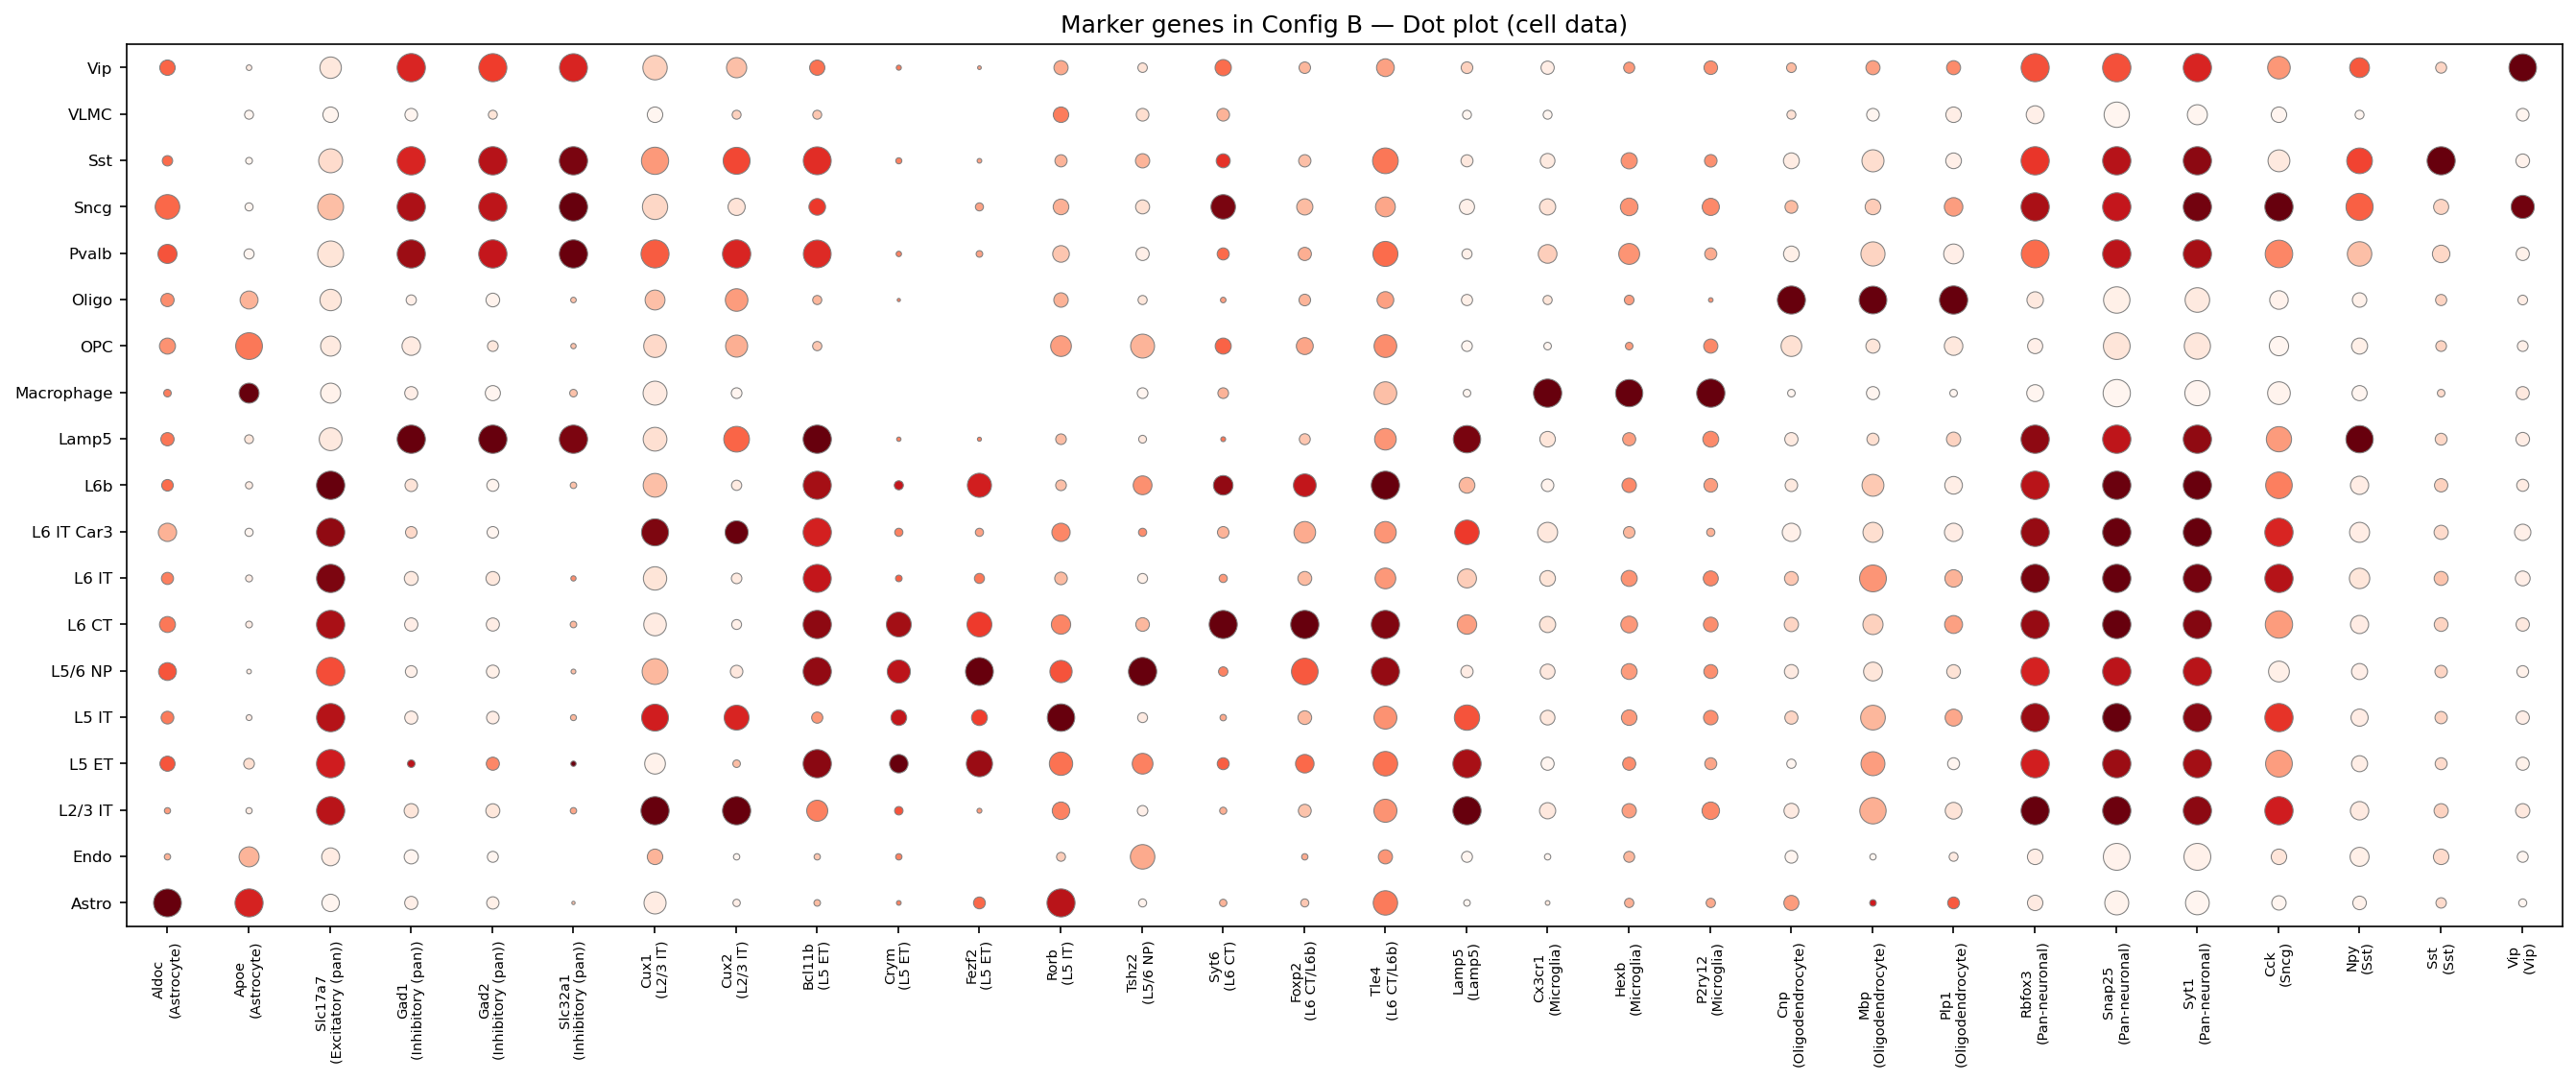
\includegraphics[width=\textwidth]{dotplot_markers.png}
\end{column}
\end{columns}
\end{frame}

% ============================================================
% SLIDE 17: PerCT fix
% ============================================================
\begin{frame}{Per-Cell-Type Filtering Recovers 58/59 Markers}

\centering
\begin{tabular}{lcccc}
\toprule
\textbf{Strategy} & \textbf{Genes} & \textbf{Markers} & \textbf{Cell Var\%} & \textbf{Nuc Var\%} \\
\midrule
Config B (current) & 10,134 & 30/59 & 85.0\% & 90.6\% \\
\textbf{PerCT 5\% (fix)} & \textbf{16,439} & \textbf{58/59} & \textbf{93.1\%} & \textbf{93.9\%} \\
\bottomrule
\end{tabular}

\vspace{1em}
\begin{itemize}
    \item Keep gene if detected in $>$5\% of \textbf{any} cell type in \textbf{either} modality
    \item Only \textit{Aldh1l1} still missing; 93\% total variance captured
    \item Stage 1 retraining in progress --- expect non-neuronal DE to improve
\end{itemize}
\end{frame}

% ============================================================
% SECTION 6: NEXT STEPS
% ============================================================
\section{Path Forward}

% ============================================================
% SLIDE 18: Per-cell variation
% ============================================================
\begin{frame}{Three Approaches to Recover Within-Cell-Type Variation}
\begin{enumerate}
    \item \textbf{Larger latent space} (32 $\to$ 64/128 dims)\\
    {\small More capacity for per-cell signal beyond cell-type identity}

    \vspace{0.3em}
    \item \textbf{Variance-preserving regularization}\\
    {\small $\mathcal{L}_{\text{var}} = \max\!\big(0,\; \tau - \text{Var}_{\text{imp}} / \text{Var}_{\text{real}}\big)$}

    \vspace{0.3em}
    \item \textbf{Read subsampling for pseudo-paired data}\\
    {\small Subsample cells $\to$ simulate nuclei $\to$ per-cell supervision}
\end{enumerate}
\end{frame}

% ============================================================
% SLIDE 19: Validation roadmap
% ============================================================
\begin{frame}{What Does This Enable? --- Validation Roadmap}
\begin{itemize}
    \item \textbf{Benchmark} vs scVI (batch correction) and per-gene linear regression
    \item \textbf{Biological test}: recover cytoplasmic markers (\textit{Fos}, \textit{Arc}) from nuclei
    \item \textbf{Human transfer}: retrain on PsychENCODE or human Allen Brain Atlas
\end{itemize}

\vspace{0.8em}
\centering
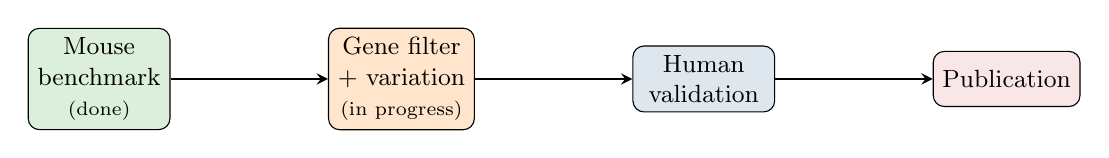
\begin{tikzpicture}[>=stealth, font=\small, node distance=2.5cm]
    \node[draw, rounded corners, fill=accentgreen!20, minimum width=1.8cm, minimum height=0.7cm, align=center] (now) {Mouse\\benchmark\\{\scriptsize (done)}};
    \node[draw, rounded corners, fill=orange!20, minimum width=1.8cm, minimum height=0.7cm, align=center, right=2cm of now] (fix) {Gene filter\\+ variation\\{\scriptsize (in progress)}};
    \node[draw, rounded corners, fill=mainblue!15, minimum width=1.8cm, minimum height=0.7cm, align=center, right=2cm of fix] (human) {Human\\validation};
    \node[draw, rounded corners, fill=accentred!15, minimum width=1.8cm, minimum height=0.7cm, align=center, right=2cm of human] (paper) {Publication};
    \draw[->, thick] (now) -- (fix);
    \draw[->, thick] (fix) -- (human);
    \draw[->, thick] (human) -- (paper);
\end{tikzpicture}
\end{frame}

% ============================================================
% SLIDE 20: Summary
% ============================================================
\begin{frame}{Three Takeaways}
\begin{enumerate}
    \item \textbf{Modality-conditioned VAE enables cross-modal imputation}\\
    {\small $r = 0.98$, +11\% classification, +5\% DE over raw nuclei}

    \vspace{0.5em}
    \item \textbf{Cross-decode nearly matches reconstruction ceiling}\\
    {\small Per-cell variance loss is a general VAE property, not cross-modal--specific}

    \vspace{0.5em}
    \item \textbf{Clear path forward}\\
    {\small PerCT gene filtering (58/59 markers), per-cell variation, human validation}
\end{enumerate}

\vspace{0.8em}
\centering
{\small
\begin{tabular}{lccc}
\toprule
& \textbf{Raw nuclei} & \textbf{Cond+XR} & \textbf{$\Delta$} \\
\midrule
Classification & 85.1\% & \textbf{95.8\%} & +10.7\% \\
DE overlap & 47.1\% & \textbf{52.1\%} & +5.0\% \\
Coexpression & 0.818 & \textbf{0.915} & +0.097 \\
\bottomrule
\end{tabular}
}
\end{frame}

% ============================================================
% THANK YOU
% ============================================================
\begin{frame}[plain]
\centering
\vspace{2cm}
{\Huge\color{mainblue} Thank you}

\vspace{1em}
{\large Questions?}

\vspace{2em}
{\small Code: \texttt{imputeVAE} on Yale HPC}
\end{frame}

\end{document}
